\documentclass[british,titlepage]{ntnuthesis}

\title{Building a Decentralized Identity Command Line Interface (DID CLI) using the Rust programming language}
\shorttitle{DID CLI}
\author{Jonas Johan Solsvik}
\shortauthor{Solsvik}
\date{CC-BY \ntnuthesisdate}


\addbibresource{thesis.bib}


% From https://www.overleaf.com/learn/latex/Glossaries

\makeglossaries % Prepare for adding glossary entries


\newglossaryentry{did-method}
{
        name=DID-method,
        plural=DID-methods,
        description={A specific type of DID. Each DID-method has it's own implementation of the DID-method operations}
}
\newglossaryentry{did-method-operations}
{
        name=DID-method Operations,
        description={Create, resolve, update, deactivate}
}
\newglossaryentry{did-key}
{
        name=did:key,
        description={The simplest DID-method. It is based on a cryptographic public-private keypair}
}
\newglossaryentry{unix}
{
        name=UNIX,
        description={A programming environment for terminals, with initial release in 1971}
}
\newglossaryentry{rust}
{
        name=Rust,
        description={A compiled, fast, safe, low-level programming language}
}
\newglossaryentry{did-kit}
{
    name=DIDKit,
    description={A cross-platform toolkit for decentralized identity, developed by Spruce ID over at https://github.com/spruceid/didkit}
}
\newglossaryentry{didcomm-rs}{
    name=DIDComm-rs,
    description={DIDComm messaging implementation in Rust, developed by DIF over at https://github.com/decentralized-identity/didcomm-rs}
}

\newglossaryentry{diwala}{
    name=Diwala,
    description={Our mission is to build an ecosystem of digital skill identities with verifiable credentials - to create global opportunities for people. About us: https://www.diwala.io/company/about-us}
}

% --------------------
% ----- Acronyms -----
% --------------------

% DID
\newacronym{ssi}{SSI}{Self-Sovereign Identity}
\newacronym{did}{DID}{Decentralized Identifier}
\newacronym{dids}{DIDs}{Decentralized Identifiers}
\newacronym{w3c}{W3C}{World Wide Web Consortium}
\newacronym{dif}{DIF}{Decentralized Identity Foundation}
\newacronym{din}{DIN}{Digital Identitet Norden}

% DIDComm
\newacronym{didcomm}{DIDComm}{DIDComm Messaging v2}
\newacronym{dcpm}{DCPM}{DIDComm Plaintext Message}
\newacronym{dcem}{DCEM}{DIDComm Encrypted Message}

% Verifiable Credentials
\newacronym{vc}{VC}{Verifiable Credentials}
\newacronym{vp}{VP}{Verifiable Presentations}
\newacronym{bdd}{BDD}{Behaviour Driven Development}

% CLI
\newacronym{cli}{CLI}{Command Line Interface}
\newacronym{gui}{GUI}{Graphical User Interface}
\newacronym{did-cli}{DID CLI}{Decentralized Identity Command Line Interface}
\newacronym{stdin}{STDIN}{Unix Standard Input}
\newacronym{stdout}{STDOUT}{Unix Standard Output}


 % add glossary and acronym lists before document

\begin{document}

\chapter*{Abstract}

Exploring our \acrfull{ssi} future, by developing a \acrfull{did-cli} - in the \gls{rust} programming language, using \gls{did-key}, \acrfull{didcomm} and \acrfull{vc}.


\tableofcontents
%\listoffigures
%\listoftables
%\lstlistoflistings

\printglossary[type=\acronymtype] % Print acronyms
\printglossary                    % Print glossary

\chapter{Introduction}



\section{Project domain - Self-Sovereign Identity (SSI)}

\paragraph{}
On April 25th 2016, Chirstopher Allen launched a blog-post laying out his vision for the future of digital identity titled "The Path to Self-Sovereign Identity"\cite{ThePathToSelfSovereignIdentity}. 

Allen's vision sees \acrfull{ssi} as the final step in the evolution of digital identity: "The models for online identity have advanced through four broad stages since the advent of the Internet: centralized identity, federated identity, user-centric identity, and self-sovereign identity."\cite{ThePathToSelfSovereignIdentity}

In the following years a whole array of new open-source technologies have initiated research and development into realizing Allen's vision. 

\acrfull{dids} is a core \acrshort{ssi}-technology, and it's \textit{design goals}\cite{DIDDesignGoals} gives us a hint about which problems \acrshort{ssi} is trying to solve:
\begin{description}
    \item["Decentralization:] Eliminate the requirement for centralized authorities or single point failure in identifier management, including the registration of globally unique identifiers, public verification keys, services, and other information."
    \item["Control:] Give entities, both human and non-human, the power to directly control their digital identifiers without the need to rely on external authorities."
    \item ["Privacy:] Enable entities to control the privacy of their information, including minimal, selective, and progressive disclosure of attributes or other data."
\end{description}

\paragraph{}
To understand this work, you should at least have a surface-level understanding of the following three core SSI-technologies - \acrfull{dids}, \acrfull{didcomm} and \acrfull{vc} - and how they relate to one another. This chapter will give you a brief summary of all three of them, beginning with \acrshort{dids}:

\newpage




\subsection{Decentralized Identifiers (DIDs)} 

According to \textit{DID Use Cases}\cite{DIDUseCases}, a \acrshort{did} is "a new type of identifier that has 4 essential characteristics:"
\begin{description}
    \item["1. decentralized:] There should be no central issuing agency;"
    \item["2. persistent:] The identifier should be inherently persistent, not requiring the continued operation of an underling organization;"
    \item["3. cryptographically verifiable:] It should be possible to prove control of the identifier cryptographically"
    \item["4. resolvable:] It should be possible to discover metadata about the identifier.
\end{description}
    
\paragraph{}
There are many different types of \acrshort{dids} that fit these characteristics. A specific type of \acrshort{did} is called a \gls{did-method}\cite{DIDMethod}. Each \gls{did-method} provides a unique specification on how to perform the different \gls{did-method-operations}\cite{DIDMethodOperations} - Create, Resolve, Update, Deactivate. 

\paragraph{}
The simplest \gls{did-method} is called \gls{did-key}\cite{DIDKey}. \gls{did-key} is created by generating a cryptographic public-private keypair on your machine, and using the public part of the keypair as a base for the DID.

\begin{lstlisting}[caption={Example of a \gls{did-key}}]
did:key:z6MkpTHR8VNsBxYAAWHut2Geadd9jSwuBV8xRoAnwWsdvktH  <--- Public key
\end{lstlisting}

If you stumble upon a \acrshort{did} in the wild, it should be easy to recognize it as a \acrshort{did}, because they all share the same signature.

\begin{lstlisting}[caption={DID-signature}]
did:<method>:<unique method-specific string of characters>
\end{lstlisting}

\begin{lstlisting}[caption={Depending on the DID-method, different DIDs may look very different from each other.}]
did:elem:EiAS3mqC4OLMKOwcz3ItIL7XfWduPT7q3Fa4vHgiCfSG2A
did:github:Caranty
did:web:identity.foundation
did:key:z6MkmjY8GnV5i9YTDtPETC2uUAW6ejw3nk5mXF5yci5ab7th
did:sov:WRfXPg8dantKVubE3HX8pw

\end{lstlisting}

As of time of writing all these \acrshort{dids} are verified to be resolveable, and you should be able to resolve them by copy-pasting them into \textit{https://dev.uniresolver.io/\cite{UniversalResolver}}.



\newpage

\subsection{DIDComm}

How \acrshort{did}-agents establish connections and pass messages with each other.


Example of a \acrfull{dcpm} \footnote{https://identity.foundation/didcomm-messaging/spec/\#plaintext-message-structure}:
\begin{lstlisting}[language=json]
{
    "id": "1234567890",
    "type": "<message-type-uri>",
    "from": "did:example:alice",
    "to": ["did:example:bob"],
    "created_time": 1516269022,
    "expires_time": 1516385931,
    "body": {
    	"messagespecificattribute": "and its value"
    }
}
\end{lstlisting}

The encrypted variant of \acrfull{dcpm} is called \acrfull{dcem}\footnote{https://identity.foundation/didcomm-messaging/spec/\#didcomm-encrypted-message}.



\subsection{Verifiable Credentials (VCs)} 

How \acrshort{did}-agents issue verifiable claims about the attributes of each other and their relationships - https://www.w3.org/TR/vc-data-model/ 

\newpage



\section{Project Scope - Agents and Wallets}

Within the \acrshort{ssi}-community there are two pieces of software that is talked about a lot - agents and wallets.


\subsection{Agents}

\begin{itemize}
    \item An agent is a piece of software that is acting on behalf of a \acrshort{did}.
    \item An agent implements one or more of the \acrshort{didcomm}-protocols.
    \item An agent is active. It wants to do things.
\end{itemize}


\subsection{Wallets}

\begin{itemize}
    \item May store \acrfull{vc}.
    \item May store a \acrshort{did}s cryptographic material.
    \item A wallet is passive. It wants to hold things.
\end{itemize}

\subsection{Agents vs Wallets}

In any \acrshort{ssi} discussion these two terms may be used interchangeably about the same piece of software. This is because many instances of \acrshort{ssi} software are both an agent and a wallet at the same time. It just depends on the context of the discussion how you will refer to the software. If the discussion is about storing credentials and your DIDs, it is more natural to think about the software as a wallet. If the discussion is about issuing, signing, communicating, transfering, validating the best metaphor is to think about the software as an agent. That is what they are - two different kinds of metaphors. Two different kind of ways to look at the same thing.




\newpage

\section{Project Initiator - Diwala}

Diwala is this projects initiator, represented by Snorre Lothar von Gohren. He is the CTO \& Co-Founder of Diwala, which is a for-profit company set out to "build an ecosystem of digital skill identities with verifiable credentials"\cite{DiwalaAbout}.

Snorre also founded \acrfull{din} - a network of organizations which "works to promote decentralized identity and highlight how individuals and society is affected by it.

\section{Project Description}

"The project ambition is to build a proof with the existing wallet standards, that it is possible to establish an open and interoperable identity wallet. Or even prove that this is not possible at this moment, because of the lack of certain standards. As part of the bachelor project team will develop a set of proof-of-concept reference implementations that can showcase the interoperability within the existing frameworks and tools that are already out there. Set together the needed pieces to prove that interoperability is possible. The reference implementation of the proof-of-concept, will prove that the user will be able to seamlessly respond to different service proof requests and issuance requests, and to be able to migrate credentials and other user-centric data stored in the users control. The work will begin with existing open source frameworks, as well as closed source service providers with good developer portals for easy testing and verification. The project is language and platform agnostic. The biggest benefit in this is to showcase that the proclaimed panacea for digital identity, is actually possible. This work will rapport on hinders, benefits and possibilities with this ecosystem, and the importance of interoperability" \cite{ProjectDescription} - \textit{Diwala}






\section{Goals}

Based on the projects description it is useful to derive a list of goals for the project:

\begin{itemize}
    \item Build a proof-of-concept \acrshort{ssi}-application that solves a real-world problem.
    \item Prove that the application is inter-operable with other existing \acrshort{ssi}-application.
\end{itemize}

\section{Boundaries}

\subsection{Organizational Boundaries}

\begin{itemize}
    \item Source-code should be open-source.
    \item Source-code should be hosted by DIN-Foundation.
\end{itemize}

\subsection{Technical Boundaries}
Some technical constraints for the proof-of-concept implementation:

\begin{itemize}
    \item Should be implemented in the Rust programming language.
    \item Use existing Rust libraries wherever possible.
    \item The application should have a \acrfull{cli}.
    \item No \acrfull{gui}.
    \item Only support one DIDComm transport: \acrshort{stdin}/\acrshort{stdout}
    \item Only support one DID-method: \gls{did-key}
    \item Only support one cryptographic-method: x25519/ed25519
    \item The source code should be open-source.
    \item The source code should be hosted by \acrshort{din}'s Github.
\end{itemize}



\section{Target audience}

\subsection{Public institutions}

We want to build the trust in SSI-infrastructure that is need for public institutions to adopt the technology.


\newpage

\section{Team Roles}

The team working on this project consists of a 1 student, 1 product owner, 2 tech supervisors and 1 academic supervisor.

\begin{table}
  \centering
  \caption{Team Roles}
  \label{tab:example1}
  \begin{tabular}{cc}
    \hline
    Name  & Role \\
    \hline
    Jonas       & Leader, Developer, Student         \\
    Snorre      & Product Owner, Tech supervisor \\
    Mariusz     & Tech supervisor \\
    Abylay      & Tech supervisor \\
    Deepti      & Academic supervisor \\
    \hline
  \end{tabular}
\end{table}



\newpage

\section{Proof-of-concept - DID CLI}

The project description demands that a proof-of-concept agent should be developed. This proof-of-concept wallet will now be referred to as \acrfull{did-cli}. Chapter 2-7 are dedicated to describe how \acrshort{did-cli} was developed. Chapter 8-9 tries to take a step back again and answers the more general questions and goals set out by the project description.

\section{Chapters Overview}

\begin{description}
    \item[Chapter 2:] Development Process - How development of \acrshort{did-cli} was managed.
    \item[Chapter 3:] Requirements - The functional and non-functional requirements of \acrshort{did-cli}.
    \item[Chapter 4:] Application Architecture - A description of the high-level design of \acrshort{did-cli}.
    \item[Chapter 5:] Command-Line Interface - A description of the user-interface of \acrshort{did-cli}.
    \item[Chapter 6:] Implementation - Details about \acrshort{did-cli} source-code.
    \item[Chapter 7:] Quality Assurance - How we test and make sure \acrshort{did-cli} does what it is supposed to do. 
    \item[Chapter 8:] Discussion - What did we decide, learn, think, feel?
    \item[Chapter 9:] Conclusion - Summary and future work.
\end{description}

\hypertarget{development-process}{%
\chapter{Development Process}\label{development-process}}

\hypertarget{kanban}{%
\section{Kanban}\label{kanban}}

To keep track of tasks we used a Kanban board.

\begin{figure}
\centering
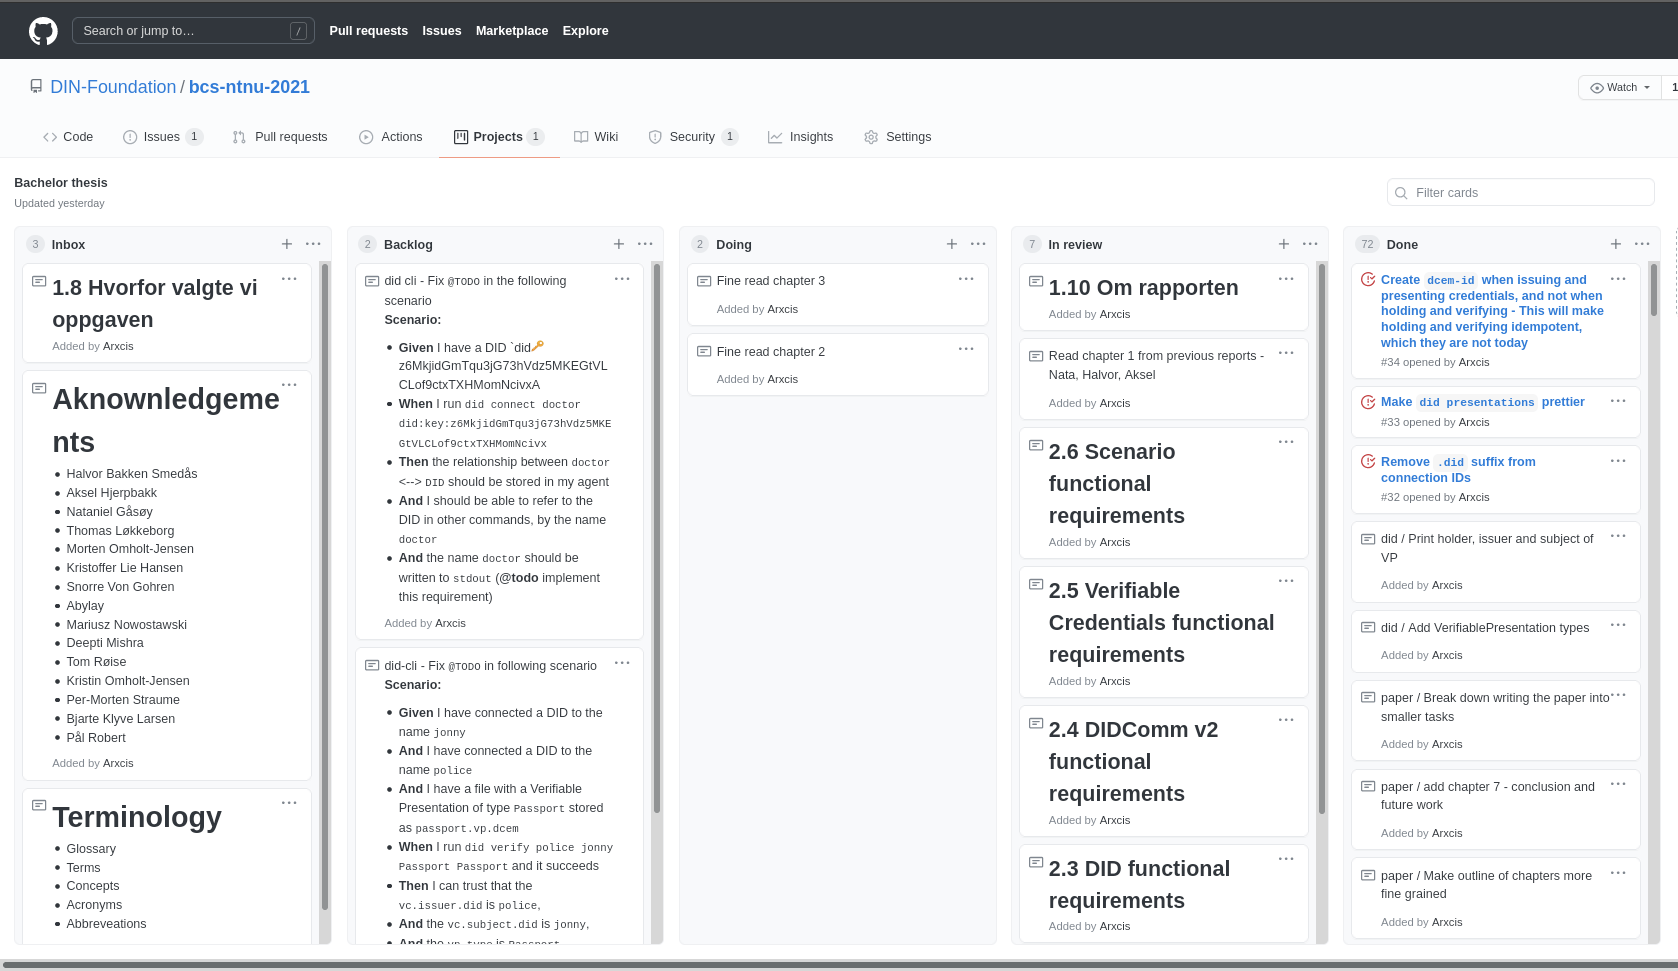
\includegraphics{Development Process a132dd5987b94adf8fc5989add9afc3f/Untitled.png}
\caption{Untitled}
\end{figure}

\hypertarget{the-5-columns-of-the-kanban-board}{%
\subsection{The 5 columns of the Kanban
board}\label{the-5-columns-of-the-kanban-board}}

\begin{enumerate}
\def\labelenumi{\arabic{enumi}.}
\tightlist
\item
  \textbf{Inbox:} List of tasks which have been thought of, but is
  lacking details like what needs to be done and when the implementation
  is supposed to happen. Tasks in backlog are created whenever someone
  feels like it. There are no requirements to put something in the
  backlog. The treshold should be as low as possible. Eqaully, the
  treshold for deleting a backlog-task should be equally low.
\item
  \textbf{Backlog:} List of tasks that are planned to be implemented in
  the near future, and have enough details ironed out to make it
  possible to start the implementation. Tasks are moved from
  \lstinline!Inbox! to \lstinline!Backlog!:

  \begin{enumerate}
  \def\labelenumii{\arabic{enumii}.}
  \tightlist
  \item
    After being discussed in the weekly domain-experts meeting.
  \item
    item or after an ad-hoc meeting dedicated to discussing a specific
    task.
  \item
    item or after the developer has researched/learned something which
    makes a task ``obviously implementable''. If a developer does this,
    it should be clearly communicated in the next weekly domain-experts
    meeting.
  \end{enumerate}
\item
  \textbf{In Progress}: List of tasks that are in progress. A developer
  have written words, code or done something else. These tasks should
  ideally be linked to an open Pull Request on Github with a WIP label
  on it.
\item
  \textbf{In Review:} List of tasks where the developer has implemented
  the task, and is waiting to get a stamp of approval from a second pair
  of eyes. Approval could be given by the client, supervisor or any of
  the domain experts. The developer will request review from the
  specific person which is considered best suited to review the pull
  request. This specific person will be notified about this on Discord,
  and via email if necessary.
\item
  \textbf{Done:} List of task where the pull request linked to the task
  has been approved and merged into the main branch of the git source
  tree.
\end{enumerate}

\pagebreak

\hypertarget{github-source-code}{%
\section{Github source code}\label{github-source-code}}

All source code is hosted at
\url{https://github.com/DIN-foundation/bcs-ntnu-2021/}.

\hypertarget{source-code-of-did-cli}{%
\subsection{Source code of DID-CLI}\label{source-code-of-did-cli}}

All DID-CLI source code was kept in a public open-source Github-repo,
during the entire development. This made it easier to collaborate on the
source code, because all participants had public access to all the work
that was being done, from day one.

\begin{figure}
\centering
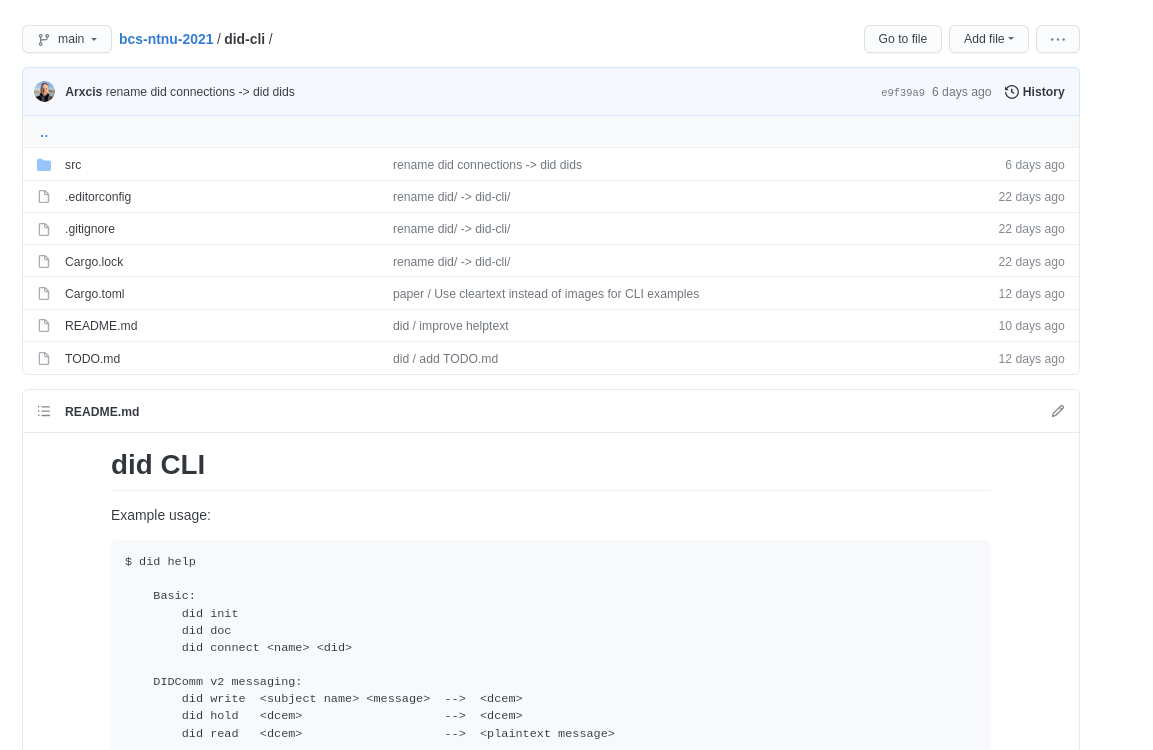
\includegraphics{Development Process a132dd5987b94adf8fc5989add9afc3f/Untitled 1.png}
\caption{Untitled}
\end{figure}

\hypertarget{source-code-of-playground-example}{%
\subsection{Source code of Playground
example}\label{source-code-of-playground-example}}

Before implementing the DID-CLI, a lot of experimentation had to be
done. This was done to learn, and iterate on smaller projects, before
beginning on the big one. Most of the projects in the playground-folder
are useless, but they served an important role as learning exercises.

\begin{figure}
\centering
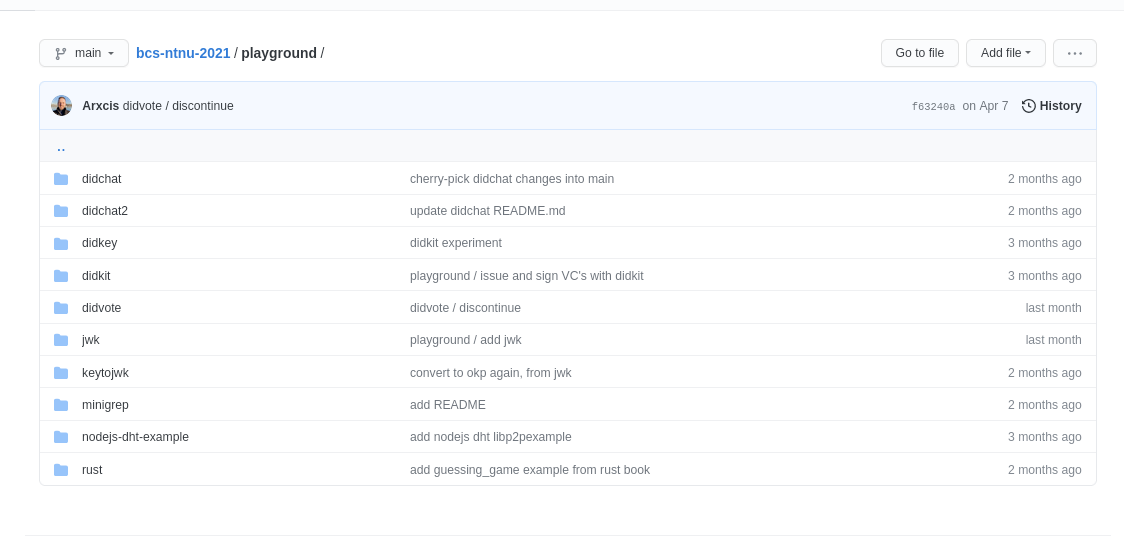
\includegraphics{Development Process a132dd5987b94adf8fc5989add9afc3f/Untitled 2.png}
\caption{Untitled}
\end{figure}

\hypertarget{source-code-of-report}{%
\subsection{Source code of Report}\label{source-code-of-report}}

Even the report was initially developed on Github, in the same repo as
DID-CLI and playground.

\begin{figure}
\centering
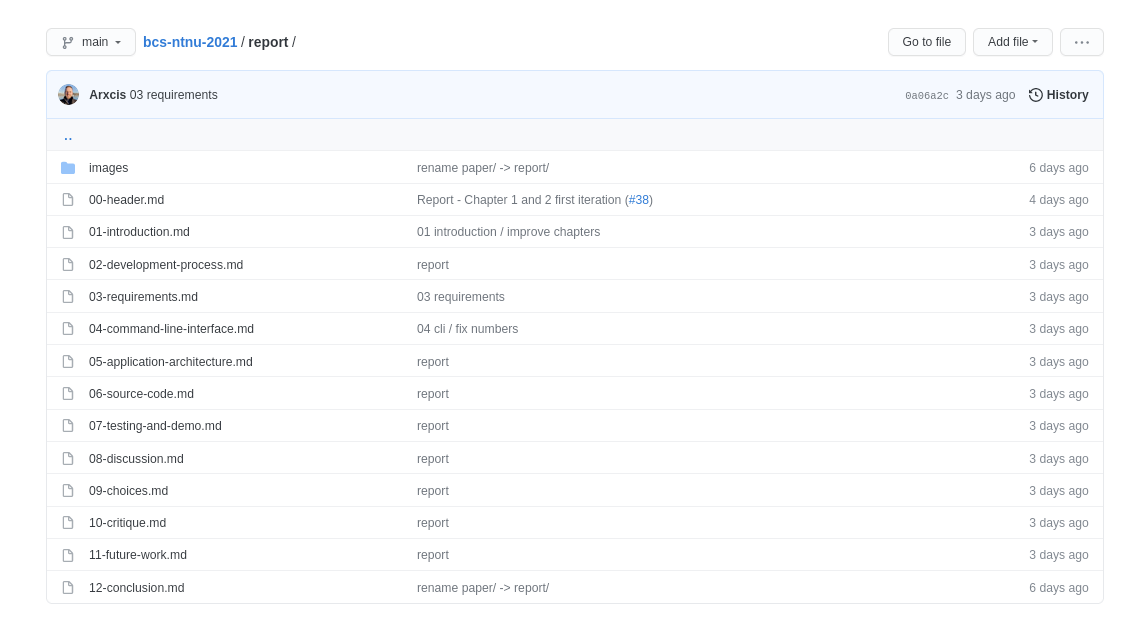
\includegraphics{Development Process a132dd5987b94adf8fc5989add9afc3f/Untitled 3.png}
\caption{Untitled}
\end{figure}

\pagebreak

\hypertarget{weekly-meetings}{%
\section{Weekly meetings}\label{weekly-meetings}}

\hypertarget{weekly-meeting-notes-on-github}{%
\subsection{Weekly meeting notes on
Github}\label{weekly-meeting-notes-on-github}}

Each meeting has a meeting note document attached to it, noting down the
attendees and a log of what was discussed during the meeting and can be
found here
\url{https://github.com/DIN-Foundation/bcs-ntnu-2021/tree/main/meetings}.

\begin{figure}
\centering
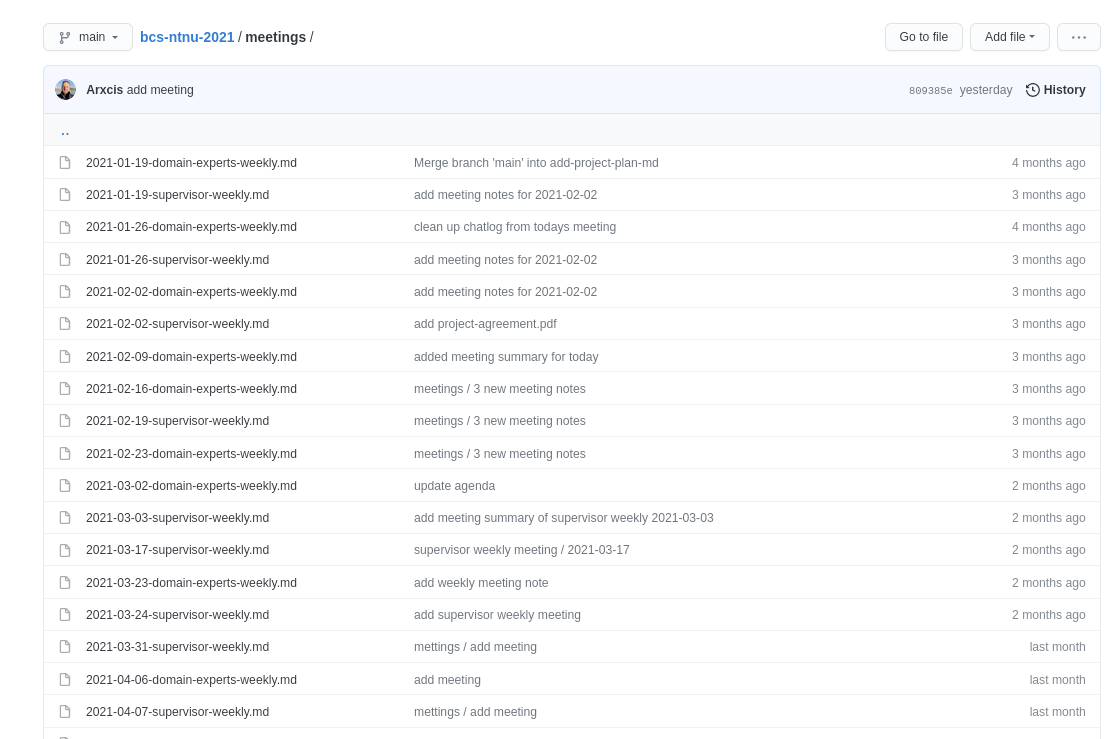
\includegraphics{Development Process a132dd5987b94adf8fc5989add9afc3f/Untitled 4.png}
\caption{Untitled}
\end{figure}

\hypertarget{domain-experts-weekly---tuesdays-1230}{%
\subsection{Domain Experts Weekly - Tuesdays @
12:30}\label{domain-experts-weekly---tuesdays-1230}}

\begin{itemize}
\tightlist
\item
  \textbf{Agenda:} Discussed questions related to the problem-domain SSI
  and software engineering. Demonstrated and validated product
  iterations.
\item
  \textbf{Attendees}: Jonas, Snorre, Mariusz, Abylay.
\item
  \textbf{Where:} Google Meet
\end{itemize}

\hypertarget{academic-supervisor-weekly---wednesdays-1400}{%
\subsection{Academic Supervisor Weekly - Wednesdays @
14:00}\label{academic-supervisor-weekly---wednesdays-1400}}

\begin{itemize}
\tightlist
\item
  \textbf{Agenda:} Discussed everything related to academic writing and
  how to organize the project's workflow.
\item
  \textbf{Attendees:} Jonas, Deepti
\item
  \textbf{Where}: Microsoft Teams
\end{itemize}

\hypertarget{a-virtual-bachelor}{%
\subsection{A virtual bachelor}\label{a-virtual-bachelor}}

Due to the pandemic, all meetings were virtual. The team never got a
chance to meet in real life during the project period. Even the final
presentation of the bachelor thesis was given over MS teams. There is no
doubt that this had a negative effect on the motivation of the student
involved in this bachelor thesis.

\pagebreak

\hypertarget{community-servers}{%
\section{Community servers}\label{community-servers}}

\textbf{DIN Discord server}

During the development process many topics were discussed inside the
DINs Discord server. This is were most of the written technical
conversations between the team members took place.

\textbf{DIF Slack server}

After a long application process which started here
\url{https://identity.foundation/join/} , I was finally accepted as a
member of the DIF foundation and allowed access to their sacred Slack
server. Here you can find many of the authors and developers of the
different SSI standards, which was an invaluable resource during the
project.

\pagebreak

\hypertarget{toggl-time-tracking}{%
\section{Toggl Time Tracking}\label{toggl-time-tracking}}

Tracking the hours was done in Toggl from day 1 (week 5), and throughout
the project (end week 20). The hours were tagged with the following 6
categories:

\begin{itemize}
\tightlist
\item
  \textbf{Meeting:} Toggled when participating in a live meeting, or
  when writing meeting notes.
\item
  \textbf{Organizing:} Toggled when organizing meetings and creating and
  updating Kanban tasks.
\item
  \textbf{Writing}: Toggled when writing the bachelor report.
\item
  \textbf{Coding}: Toggled when coding in the playground mini-projects,
  or the DID-CLI main project.
\item
  \textbf{Researching}: Toggled when reading specifications, papers,
  blog-posts, discussing with experts on the DIF and DIN slack/Discord
  channels, watching videos, reading previous bachelor reports, reading
  books, and more\ldots{}
\item
  \textbf{Lecture}: Toggled when participating in weekly lectures in the
  profprog-course, or one of the ``lightning lectures'' related to the
  bachelor-course.
\end{itemize}

\emph{Example 1: Toggl live calendar}

\begin{figure}
\centering
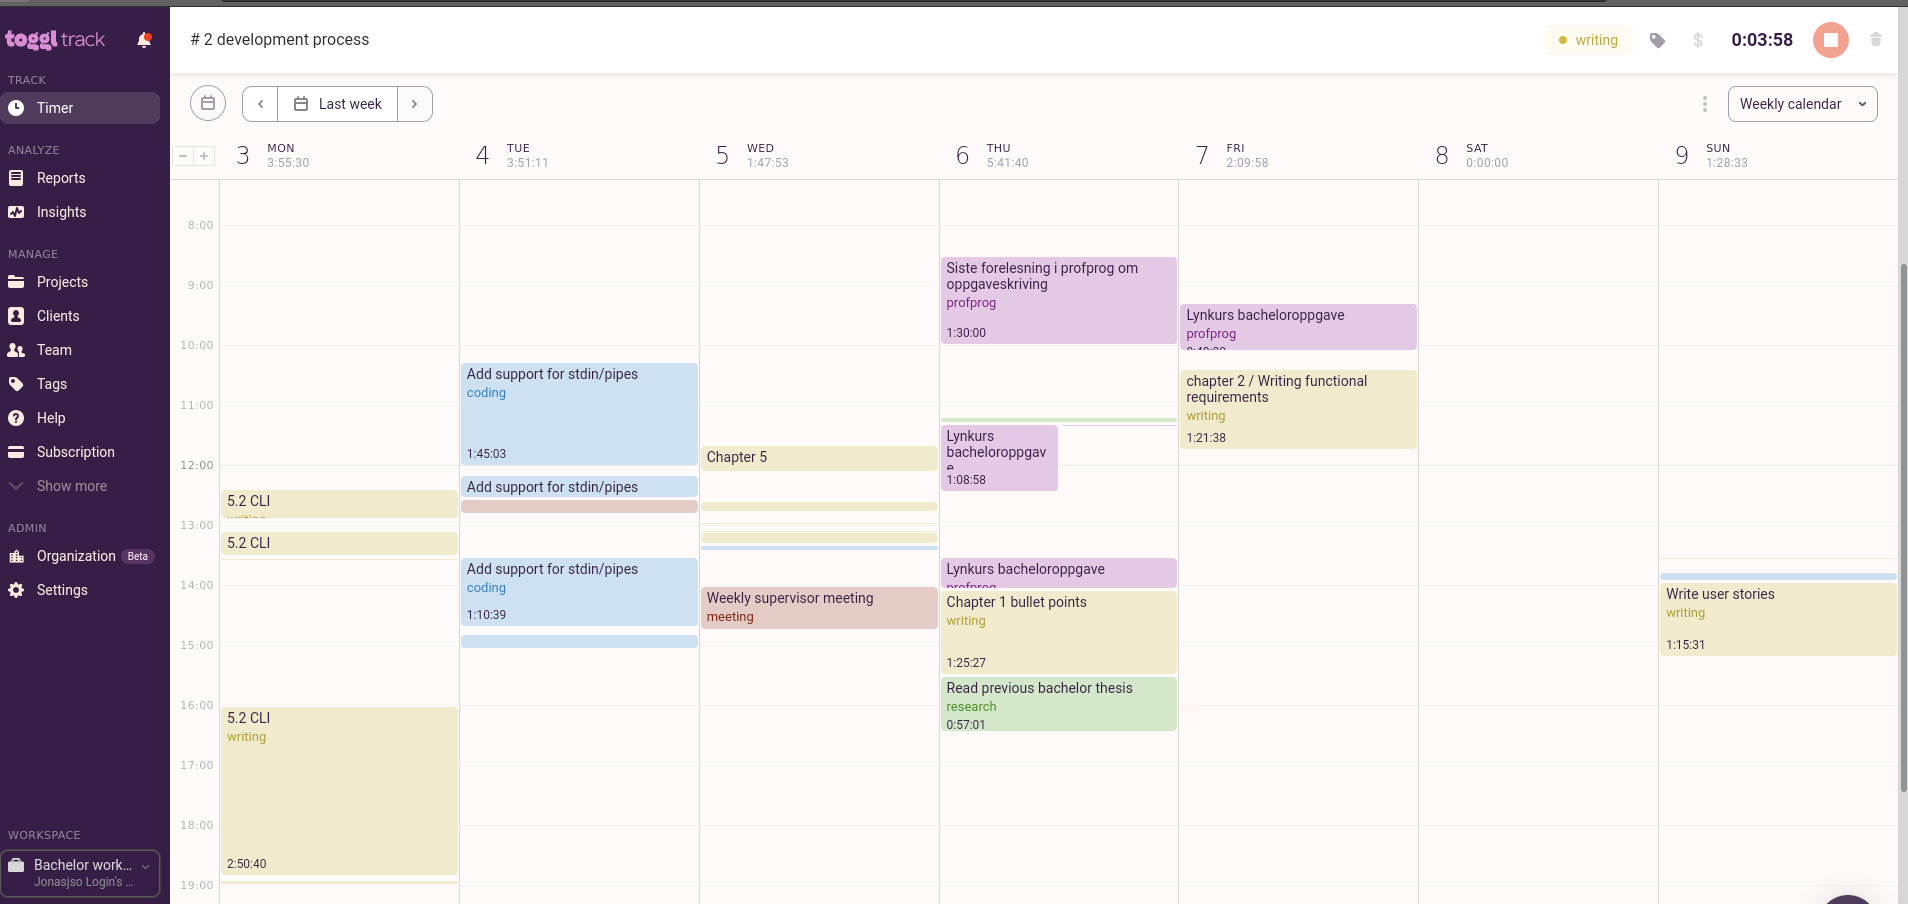
\includegraphics{Development Process a132dd5987b94adf8fc5989add9afc3f/Untitled 5.png}
\caption{Untitled}
\end{figure}

\emph{Example 2: Toggl report}

\begin{figure}
\centering
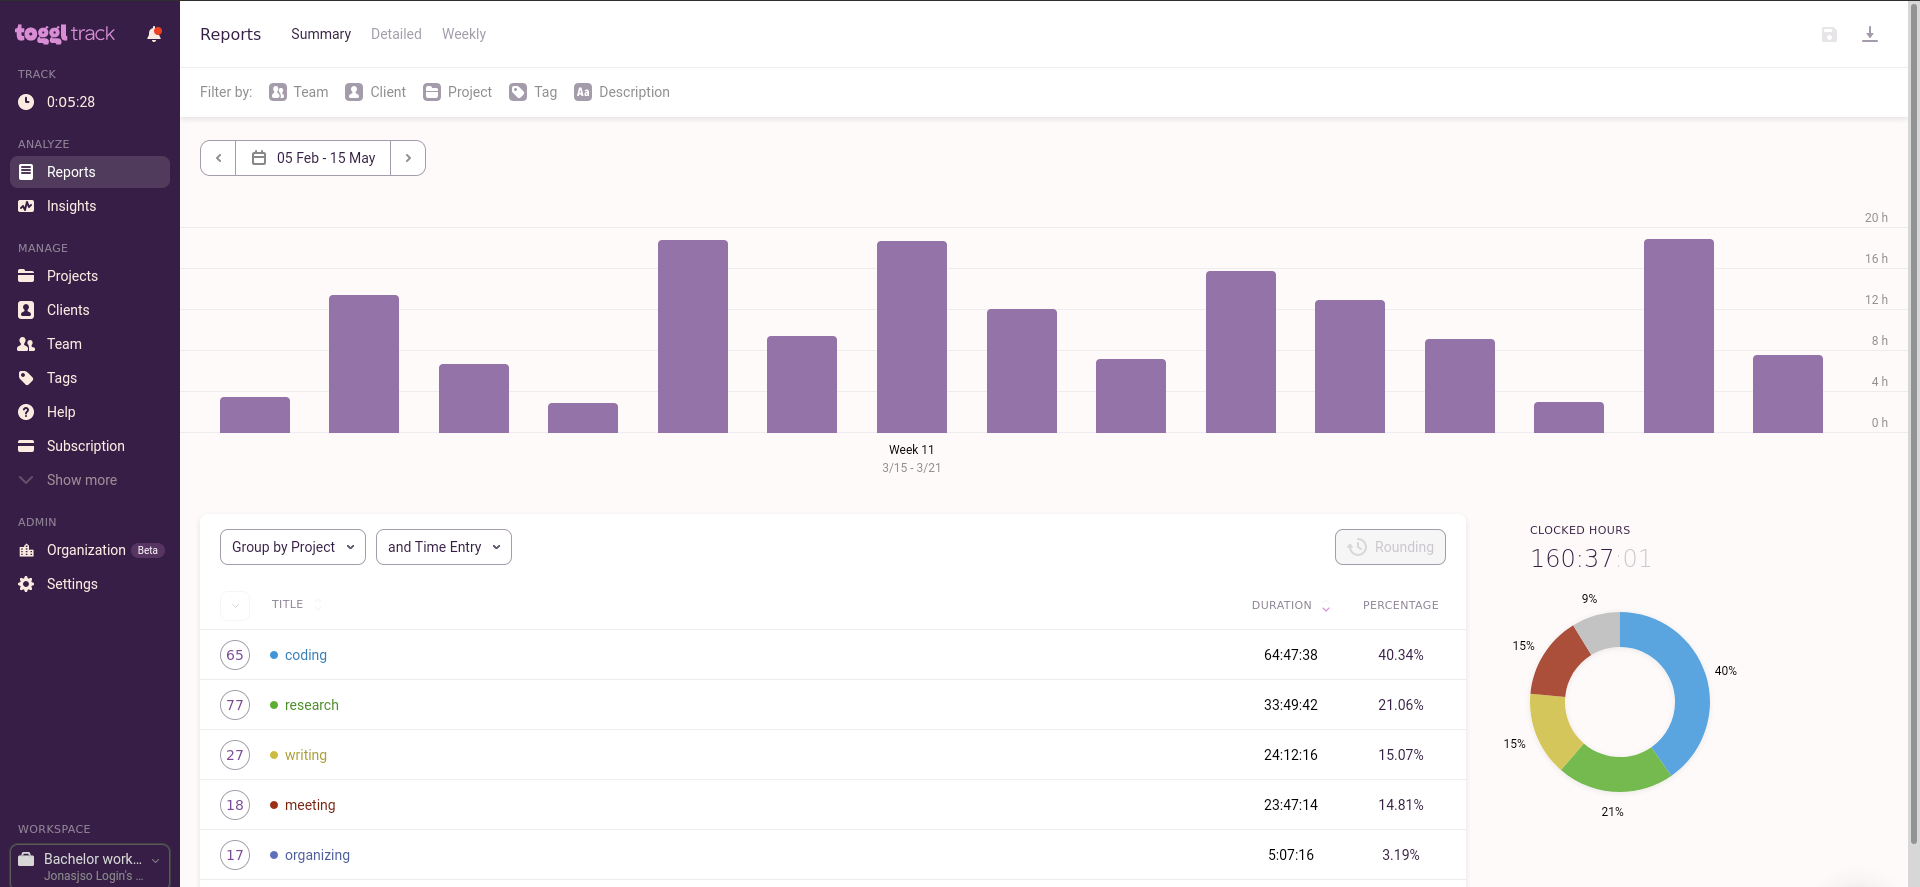
\includegraphics{Development Process a132dd5987b94adf8fc5989add9afc3f/Untitled 6.png}
\caption{Untitled}
\end{figure}

\chapter{Functional Requirements}

This chapter contains a detailed analysis of the functional requirements of \acrshort{did-cli}.

\section{Real world scenario}

\paragraph{}
To motivate the development of \acrshort{did-cli}'s requirements we want to define a real-world scenario which \acrshort{did-cli} should be the solution to. The real-world scenario depicted below is just for demonstration purposes and not an actual scenario:

\paragraph{}
\textit{The norwegian drivers license issuer, Statens Vegvesen, is considering to start issuing it's drivers licenses as \acrfull{vc}s. Statens Vegvesen is not sure if \acrshort{vc}s are the future yet, but are willing to try and dip it's toes into the water.}

\paragraph{}
\textit{What Statens Veivesen want is a proof-of-concept to be developed, which will issue, hold and verify driver-licenses as \acrfull{vc}s. The proof-of-concept should demonstrate how it handles a situation were a driver is pulled over by the police.}


    \begin{figure}[htbp]
      \centering
      
\includegraphics[width=.65\textwidth]{figures/politikontrollnrk.jpg}
      \caption[]{Driver pulled over by the police - nrk.no}
    \end{figure}




\newpage

\section{Functional Requirements Writing Style}

The functional requirement are written with User-Stories templates as titles and with \acrfull{bdd} templates as descriptions.


\section{Functional Requirement Layers}

The functional requirements are grouped together in 4 groups. Each group represents a layer in the \acrshort{ssi}-stack.
\begin{description}
    \item[Layer 1:] \acrfull{did}
    \item[Layer 2:] \acrfull{didcomm}
    \item[Layer 3:] \acrfull{vc}
    \item[Layer 4:] Application (User story)
\end{description}



\newpage

\section{Functional Requirements Layer 1 - DID}


\subsection{As a user I want to create a agent inside a directory on my machine}
\begin{description}
    \item[Given] I am in an empty directory
    \item[When] I run \texttt{did init}
    \item[Then] an agent should be created in the directory
    \item[and] all the agent's files should be stored in the sub-directory .did/, like .git/
    \item[and] the agent's DID should be written to stdout 
    \item[and] a the DIDName \texttt{self} should be linked to the DID
    \item[and] the directory is now of the type "agent-directory".
\end{description}


\subsection{As a user I want to view an agent's DID}
\begin{description}
    \item[Given] I am in an agent-directory
    \item[When] I run \texttt{did init}
    \item[or] I run \texttt{did did self}
    \item[Then] the agent's DID should be written to \texttt{stdout}.
\end{description}


\subsection{As a user I want to view an agent's DID document}
\begin{description}
    \item[Given] I am in an agent-directory
    \item[When] I run \texttt{did doc}
    \item[Then] the agent's DID-document should be written to \texttt{stdout} as prettified JSON.
\end{description}


\subsection{As a user I want to connect a name to a DID}
\begin{description}
    \item[Given] I am in an agent-directory
    \item[and] I have a DID \texttt{did:key:z6MkjidGmTqu3jG73hVdz5MKEGtVLCLof9ctxTXHMomNcivxA}
    \item[When] I run \texttt{did connect doctor did:key:z6MkjidGmTqu3jG73hVdz5MKEGtVLCLof9ctxTXHMomNcivx}
    \item[Then] the name \texttt{doctor} should be stored in the agent
    \item[and] I should be able to use \texttt{doctor} in other commands, instead of typing the whole underlying DID.
    \item[and] the name \texttt{doctor} should be written to \texttt{stdout}, to enable chaining together commands.
\end{description}


\subsection{As a user I want to refer to an agent's DID by using the name self}
\begin{description}
    \item[Given] I am in an agent-directory
    \item[When] I run any command. Example: \texttt{did write self hello}
    \item[Then] I should be able to refer to the agents own DID by the name \texttt{self}.
\end{description}


\subsection{As a user I want to view all my DID's}
\begin{description}
    \item[Given] I am in an agent-directory
    \item[and] I there are some DIDNames stored in the agent
    \item[When] I run \texttt{did dids}
    \item[Then] a list of all the agent's DIDNames should be written to `stdout`.
\end{description}


\subsection{As a user I want to view a DIDName's DID}
\begin{description}
    \item[Given] I am in an agent-directory
    \item[and] the agent has a DIDName \texttt{police}
    \item[When] I run \texttt{did did police}
    \item[Then] the DID of \texttt{police} should be written to \texttt{stdout}.
\end{description}


\newpage

\section{Functional Requirements Layer 2 - DIDComm}

\subsection{As a user I want to write a DCEM from one agent to another}

\begin{description}[1.35cm]
    \item[Given] I have two agents on my machine
    \item[and] I am in one of the agent-directories
    \item[and] I have stored the DID of the other agent by the name \texttt{other}
    \item[When] I run \texttt{did write other hello}, with the contents "Hello".
    \item[Then] a DCEM should be written to \texttt{stdout}
    \item[and] the DCEM should be addressed to \texttt{other}. 
\end{description}

For more info on DCEM - DIDComm Encrypted Message - see: https://identity.foundation/didcomm-messaging/spec/\#didcomm-encrypted-message.



\subsection{As a user I want to read the contents of a DCEM addressed to an agent}
\begin{description}[1.35cm]
    \item[Given] I am in an agent-directory
    \item[and] I receive a DCEM-file - \texttt{hello.dcem} - addressed to my agent
    \item[When] I run \texttt{did read \$(cat hello.dcem)} 
    \item[or] I run \texttt{cat hello.dcem | did read}
    \item[Then] the plaintext contents of the DCEM should be written to \texttt{stdout}.
\end{description}



\subsection{As a user I want to hold a DCEM inside an agent}
\begin{description}[1.35cm]
    \item[Given] I am in an agent-directory
    \item[and] I receive a DCEM-file - \texttt{hello.dcem} - addressed to my agent
    \item[When] I run \texttt{did hold \$(cat hello.dcem)} 
    \item[or] I run \texttt{cat hello.dcem | did hold}
    \item[Then] the DCEM should be stored inside my agent with the id of the DCEM
    \item[and] the DCEM should be written to `stdout`.
\end{description}

Note: If an existing DCEM has id=4, and a new DCEM also has id=4, then new DCEM should overwrite the one already held by the agent.



\subsection{As a user I want to view a list of all DCEMs an agent is holding}
\begin{description}[1.35cm]
    \item[Given] I am in an agent-directory
    \item[and] the agent is holding multiple DCEMs
    \item[When] I run \texttt{did messages}
    \item[Then] a list of all agent's DCEM-ids, should be written to \texttt{stdout}.
\end{description}



\subsection{As a user I want to view a single DCEM an agent is holding}
\begin{description}[1.35cm]
    \item[Given] I am in an agent-directory
    \item[and] there is a DCEM with id \texttt{7497036273686508746}, held by the agent
    \item[When] I run \texttt{did message 7497036273686508746}
    \item[Then] the DCEM should be written to \texttt{stdout}.
\end{description}



\newpage



\section{Functional Requirements Layer 3 - Verifiable Credentials}



\subsection{As an issuer I want to issue a Verifiable Credential to a subject}
\begin{description}[1.35cm]
    \item[Given] I am in an agent-directory
    \item[and] the agent has connected a DID to the name \texttt{bob}
    \item[When] I run \texttt{did issue Passport bob}
    \item[Then] a DCEM with a Verifiable Credential of type \texttt{Passport}, with \texttt{vc.subject.did} of \texttt{bob}, and with \texttt{vc.issuer.did} of \texttt{self}, should be written to \texttt{stdout}.
\end{description}



\subsection{As a holder I want to present a Verifiable presentation to a verifier}
\begin{description}[1.35cm]
    \item[Given] I am in an agent-directory
    \item[and] the agent has connected a DID to the name \texttt{police}
    \item[and] the agent is holding a Verifiable Credential as a DCEM with id 1234
    \item[When] I run \texttt{did message 1234 | did present police}
    \item[or] I run \texttt{did present Passport police \$(did message 1234)}
    \item[Then] a DCEM with a Verifiable Presentation of type \texttt{Passport}, containing the Verifiable Credential from \texttt{did message 1234}, with \texttt{vp.holder.did} of \texttt{self}, should be written to \texttt{stdout}.
\end{description}



\subsection{As a verifier I want to verify a Verifiable Presentation}
\begin{description}[1.35cm]
    \item[Given] I am in an agent-directory
    \item[and] and the agent has connected a DID to the name \texttt{jonny}
    \item[and] and the agent has connected a DID to the name \texttt{police}
    \item[and] I have a file with a Verifiable Presentation of type \texttt{Passport}, stored as \texttt{passport.vp.dcem}
    \item[When] I run \texttt{cat passport.vp.dcem | did verify Passport police jonny}
    \item[or] I run \texttt{did verify Passport police jonny \$(cat passport.vp.dcem)}
    \item[and] it succeeds
    \item[And] I can trust that the\texttt{vp.type} is \texttt{Passport}
    \item[Then] I can trust that the \texttt{vp.vc.issuer.did} is \texttt{police}
    \item[And] I can trust that the \texttt{vp.vc.subject.did} is \texttt{jonny}
    \item[And] I the file \texttt{passport.vp.dcem} will be written to \texttt{stdout}.
\end{description}



\newpage



\section{Functional Requirements Layer 4 - Scenario}



\subsection{As a citizen I want to publish my DID to a directory other citizens can access}
\begin{description}[1.35cm]
    \item[Given] I am in my agent's directory
    \item[When] I run \texttt{did init > ../jonas.did}
    \item[or] I run \texttt{did did self > ../jonas.did}
    \item[Then] a file with the name \texttt{../jonas.did} should contain my DID.
\end{description}



\subsection{As a government I want to connect to my citizens' agents}
\begin{description}[1.35cm]
    \item[Given] I am in my agent's directory
    \item[and] my citizens each have their own agents
    \item[and] each citizen have published their DID as files \texttt{../snorre.did}, \texttt{abylay.did}, \texttt{jonas.did}
    \item[When] I run \texttt{cat jonas.did | did connect jonas}
    \item[and] I run \texttt{cat abylay.did | did connect abylay}
    \item[and] I run \texttt{cat snorre.did | did snorre snorre}
    \item[Then] I should be able to refer to my citizens by the names \texttt{jonas}, \texttt{abylay} and \texttt{snorre}, in other commands.
\end{description}



\subsection{As a citizen I want to connect to my governemnt DID}
\begin{description}[1.35cm]
    \item[Given] I am in my agent's directory
    \item[and] my governemnt has a DID published in the file \texttt{../government.did}
    \item[When] I run \texttt{cat governemnt.did | did connect government}
    \item[Then] I should be able to refer to the name \texttt{government} in other commands.
\end{description}



\subsection{As government I want issue Passports to my citizens as files}
\begin{description}[1.35cm]
    \item[Given] I am in my agent's directory
    \item[and] my country has 3 citizens 
    \item[and] I have connected to my citizens
    \item[When] I run \texttt{did issue Passport jonas > ../jonas.passport.vc.dcem}
    \item[and] I run \texttt{did issue Passport abylay > ../abylay.passport.vc.dcem}
    \item[and] I run \texttt{did issue Passport snorre > ../snorre.passport.vc.dcem}
    \item[Then] All my citizens should have access to a passport issued by me
    \item[and] one citizen should only be able to use the passport issued to him/her
    \item[and] one citizen should not be able to use the passport to issued others.
\end{description}



\subsection{As a citizen I want to hold Passports issued to me}
\begin{description}[1.35cm]
    \item[Given] I am in my agent's directory
    \item[and] my government has issued a Passport to in a file \texttt{../jonas.passport.vc.dcem}
    \item[When] I run \texttt{cat ../jonas.passport.vc.dcem | did hold}
    \item[Then] the Passport is stored in my agent as a DCEM.
\end{description}



\subsection{As a citizen I want to view my Passport in plaintext}
\begin{description}[1.35cm]
    \item[Given] I am in my agent's directory
    \item[and] I have am holding a Passport as a DCEM with id 1234
    \item[When] I run \texttt{did message 1234 | did read}
    \item[Then] my Passport should be written to \texttt{stdout} in plaintext.
\end{description}



\subsection{As a citizen I want to present my Passport to the Police}
\begin{description}[1.35cm]
    \item[Given] I am in my agent's directory
    \item[and] I have am holding a Passport as a DCEM with id 1234
    \item[and] I have connected a DID to the name \texttt{police}
    \item[When] I run \texttt{did message 1234 | did present police > ../jonas.passport.vp.dcem}
    \item[Then] my Passport should be stored in a file as a Verifiable Presentation
    \item[and] it should only be able to be viewed and verified by \texttt{police}
    \item[and] nobody else.
\end{description}



\subsection{As the Police I want to verify a Passport from a citizen I am controlling}
\begin{description}[1.35cm]
    \item[Given] I am in my agent's directory
    \item[and] I have approached a citizen which has a agent
    \item[and] the citizens DID is stored in my agent with name \texttt{jonas}
    \item[and] the government's DID is stored in my agent with name \texttt{government}
    \item[and] the citizen presents his passport to me as the file \texttt{../jonas.passport.vp.dcem}
    \item[When] I run \texttt{cat ../jonas.passport.vp.dcem | did verify Passport government jonas}
    \item[Then] I can be sure that Verifiable Presentation is of type \texttt{Passport}
    \item[and] and is issued by the \texttt{government}
    \item[and] and has a subject of \texttt{jonas}
\end{description}


\chapter{Application Architecture}

\section{Data Model}



\subsection{DID, DID Document and DID-methods}
\begin{itemize}
\item A DID is the unique identifier of an agent.
\item DID's can resolve to a DID Document.
\item The DID-method decides the details on how to resolve the DID-document.
\item DID data model -> https://www.w3.org/TR/did-core/\#data-model
\end{itemize}



\subsection{DIDKey method}

DIDKey is the only DID-method we are supporting. DID method key format -> https://w3c-ccg.github.io/did-method-key/\#format



\subsection{ed25519-JWK}

The JWK DID-CLI is supporting, is a `ed25519/x25519` cryptographic public-private keypair, underpinning the DIDKey-method. The `jwk` is used for many things:
\begin{itemize}
\item Each unique `jwk` maps to a unique DID in the DIDKey-method.
\item By holding the `jwk`, the agent is able to assert control over it's DID in the DIDKey-method.
\item The `jwk` is used to encrypt DIDComm messages.
\item The `jwk` is used when generating the shared key in the Elliptic-Curve-Diffie-Helmann-key-exchange (ECDH-protocol).
\item The `jwk` is used to sign Verifiable Credentials and Verifiable Presentations.
\end{itemize}

\newpage

\begin{lstlisting}[
    caption={Example of an ed25519-jwk},
    label=lst:json,
    language=json]
{
	"kty":"OKP",
	"crv":"Ed25519",
	"x":"YRJAoEuAzcdc_7QdEM0NHQCd6hd-FdHkpdXl8T-RlVA",
	"d":"HOrwgKInYvPw_Wh6nN6kTNEd3wkkwYySMSuXzdr5Gec"
}
\end{lstlisting}

JWK format -> https://datatracker.ietf.org/doc/html/rfc7517\#section-4.1



\subsection{DCEM - DIDComm Encrypted Message}

All messages read and written by the agent, are serialized as DIDComm Encrypted Messages, both in transit, and when at stored at rest inside the agent, as files.

DCEM spec -> https://identity.foundation/didcomm-messaging/spec/\#didcomm-encrypted-message



\subsection{Verifiable Credentials}

All credentials issued by DID CLI are serialized as Verifiable Credentials.

    \begin{figure}[htbp]
      \centering
      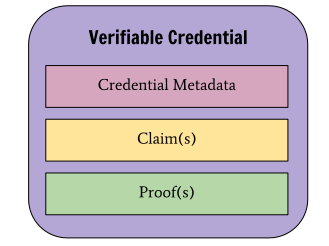
\includegraphics[width=.7\textwidth]{figures/credential.png}
      \caption[]{Illustration from https://www.w3.org/TR/vc-data-model/\#credentials}
    \end{figure}



\newpage

\subsection{Verifiable Presentations}

All presentations presented by DID CLI are serialized as Verifiable Presentations.
    
    \begin{figure}[htbp]
      \centering
      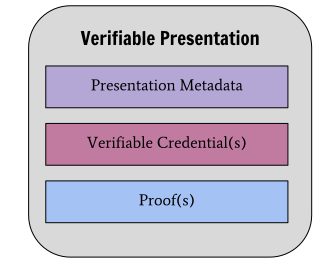
\includegraphics[width=.7\textwidth]{figures/presentation.png}
      \caption[]{Illustration from https://www.w3.org/TR/vc-data-model/\#presentations}
    \end{figure}
    


\subsection{DIDName}
\begin{itemize}
    \item DIDName is a way of refering to a DID in a local DID-CLI command, because it is impossible to remember the full DID.
    \item DIDName is the only part of DID-CLI's data-model which is not part of an SSI-standard.
    \item Each DIDName is stored as a file `<DIDName>.did`, and the full DID as the content.
    \item Example: `self.did` or `jonas.did`.
\end{itemize}




\newpage


\section{File Storage}

\subsection{The .did/-directory}

All the agents files are contained within the `.did/`-directory, created when initializing the agent. The DID-CLI will use whatever `.did/`-directory is inside the current terminal working directory, just like GIT-CLI uses the `.git/`-directory.

\subsection{Portability}

The agent database, represented by the `.did/` directory, should be portable. A user should be able to move it to any other location on local machine, or to any other machine, and the agent should still work.


\subsection{One directory per agent}

\begin{lstlisting}[language=bash,caption={bash version}]

for i in bob lisa snorre jonas
do
	mkdir $i;
	cd $i;
	did init;
	cd ..;
done
\end{lstlisting}




\subsection{Communicating by sharing files}

\begin{lstlisting}[language=bash,caption={bash version}]
mkdir bob/ lisa/
cd bob/
did init
did did self > ../bob.did

cd ../lisa
did init
did did self > ../lisa.did

cd ../lisa
cat ../bob.did | did connect bob
cd ../bob
cat ../lisa.did | did connect lisa
\end{lstlisting}



\newpage


\section{High-level flow of scenario}

\subsection{Part 1 - The Government Issues credentials to it's citizens}


    \begin{figure}[htbp]
      \centering
      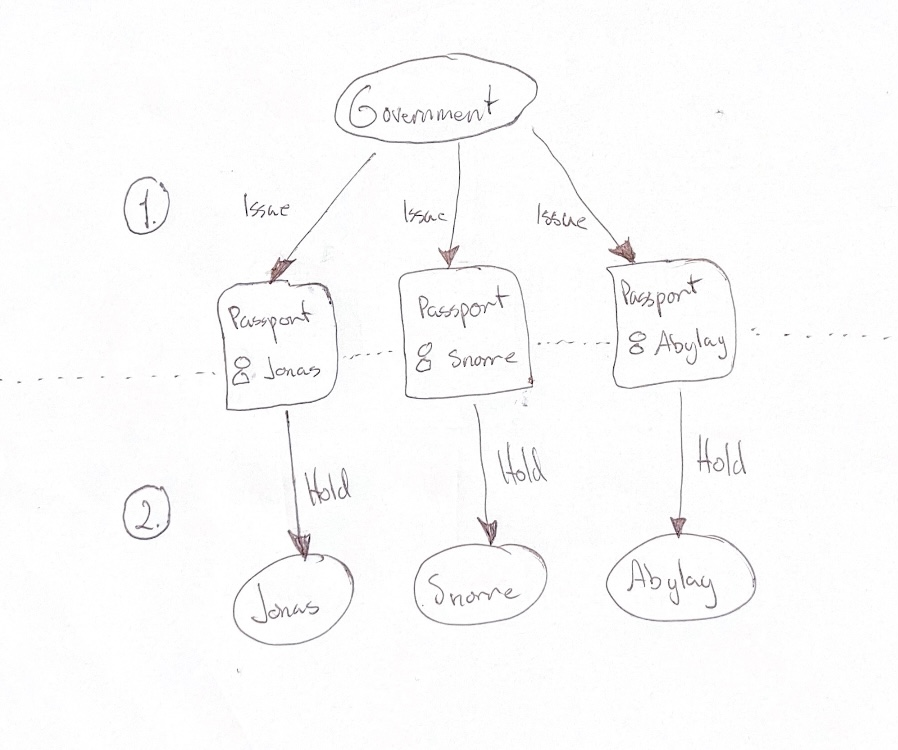
\includegraphics[width=.5\textwidth]{figures/scenario-1-2.png}
      \caption[]{Scenario Part 1 - Action 1 and 2}
    \end{figure}


\begin{description}
    \item[1. Issue:] The Government-agent issues 3 passport as Verifiable Credentials, to the 3 different citizen-agents - Jonas, Snorre and Abylay.
    \item[2. Hold:] The 3 citizen agents each hold the one passport issued to them.
\end{description}

    \begin{figure}[htbp]
      \centering
      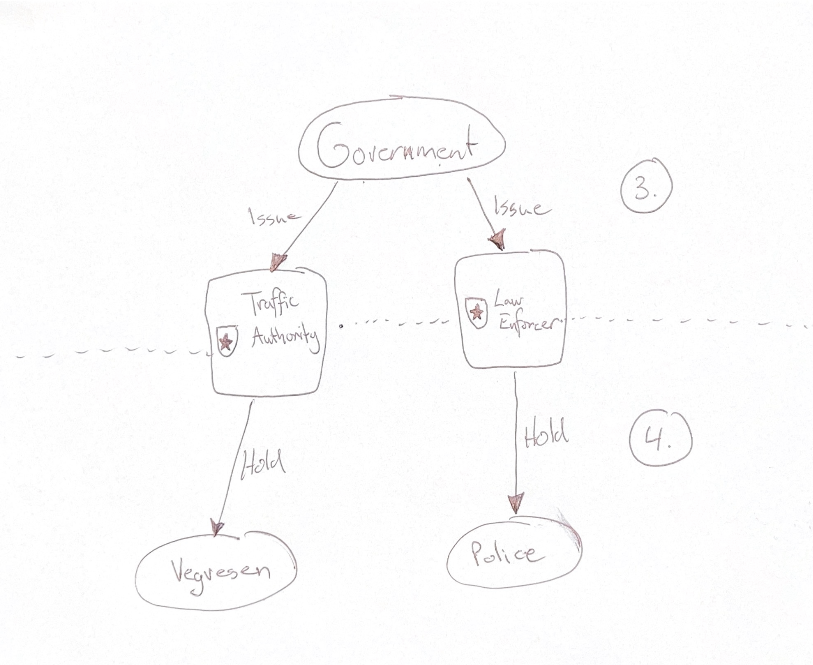
\includegraphics[width=.5\textwidth]{figures/scenario-3-4.png}
      \caption[]{Scenario Part 1 - Action 3 and 4}
    \end{figure}

\begin{description}
    \item[3. Issue:] The Govenment-agent issues a Traffic Authority and a Law Enforcer credential, to two different agents. This, in practice, creates the "Vegvesen" and the Police.
    \item[4. Hold:]The "Vegvesen"-agent and the Police-agent holds their respective credentials issued to them.
\end{description}


\newpage

\subsection{Part 2 - Jonas gets a Drivers License from Vegvesen}

    \begin{figure}[htbp]
      \centering
      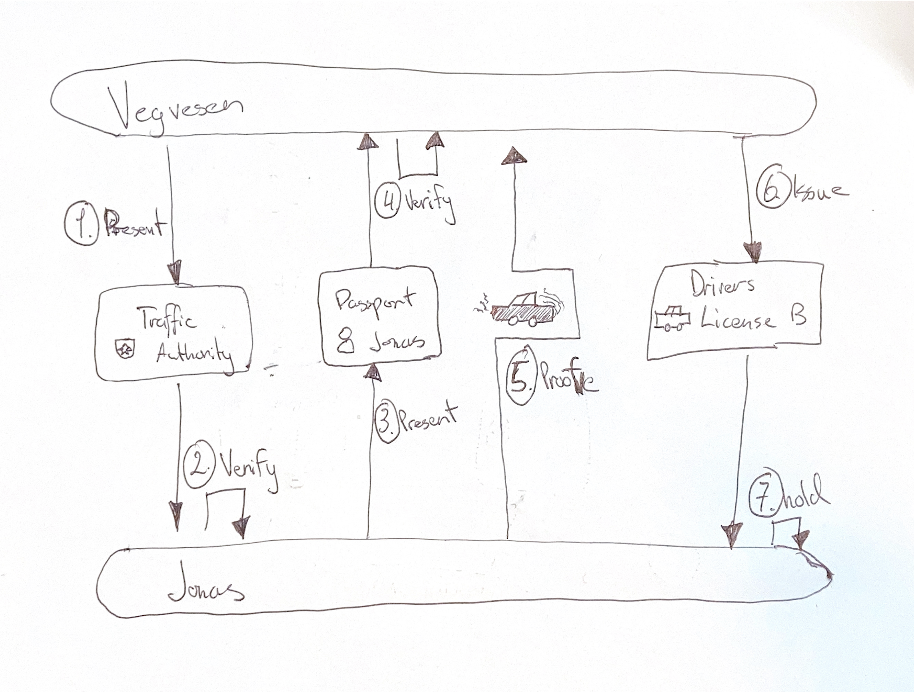
\includegraphics[width=1\textwidth]{figures/scenario-part2.png}
      \caption[]{Scenario Part 2}
    \end{figure}
    
\begin{description}
\item[1. Present:] - Vegvesen presents it's "Traffic Authority"-credential to Jonas,.
\item[2. Verify:] - Jonas verifies that the presentation has a valid signature, and makes sure that the "Traffic Authority"-credential was signed by the Government.
\item[3. Present:] - Jonas presents his "Passport"-credential to Vegvesen.
\item[4. Verify:] - Vegvesen verifies that the presentation is valid, and makes sure the passport credential was signed by the Government.
\item[5. Proove:] - Jonas somehow proves to Vegvesen that he know how to drive a car. This is out of scope of any of the SSI-protocols.
\item[6. Issue:] - Vegvesen issues a Drivers License as a Verifiable Credential to Jonas.
\item[7.  Hold:] - Jonas holds the Drivers License issued to him.
\end{description}


\newpage

\subsection{Part 3 - Jonas presents his Drivers License to Police}

    \begin{figure}[htbp]
      \centering
      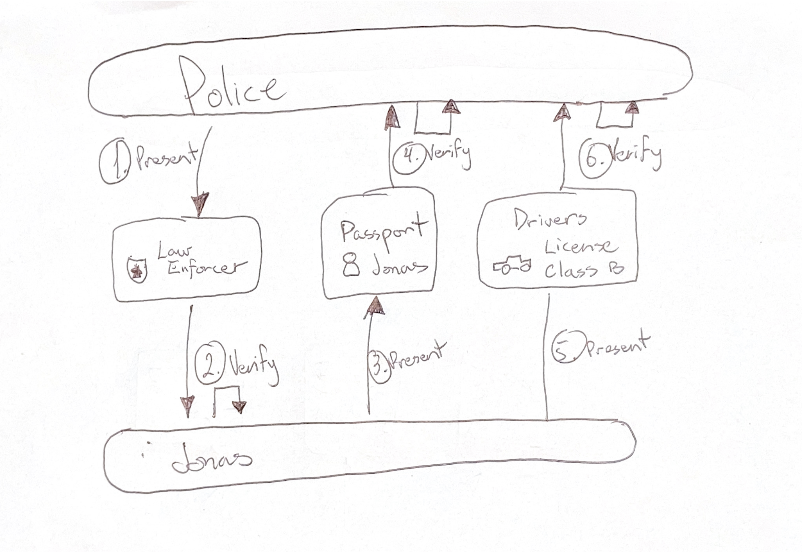
\includegraphics[width=1\textwidth]{figures/scenario-part3.png}
      \caption[]{Scenario Part 3}
    \end{figure}

\begin{description}
    
    \item[1. Present:] Police presents it's "Law Enforcer"-credential to Jonas.
    \item[2. Verify:] Jonas verifies that the presentation has a valid signature, and makes sure that the "Traffic Authority"-credential is issued by the Government.
    \item[3. Present:] Jonas presents it's Passport-credential to the Police.
    \item[4. Verify:] Police verifies that the presentation has a valid signature, and makes sure that the Passport-credential is issued by the Government.
    \item[5. Present:] Finally Jonas presents his Drivers License.
    \item[6. Verify:] Police verifies that the Drivers License is valid, and issued by the Government.
\end{description}

\chapter{Command-Line Interface}

\begin{itemize}
\item The main way to interact with `did` executeable, is through it's CLI.
\item Each command follows the same pattern `did <command> <...args>`.
\item The DID-CLI draws inspiration from the book `The Unix Programming environment` by `Brian W. Kernighan` and `Rob Pike`, 1984.
\end{itemize}

\section{Unix Pipelines Integration}

Many of the commands in the DID-CLI, is designed in a way to easily integrate with existing Unix tools. The most important part of this integration, is to support optionally reading input from `stdin`. Also it is important to take care in how output is written to `stdout`, to make it possible to chain commands together. This is the reason you will see that most of commands are standardized to write full DCEM-messages to `stdout`, for easy consumption by the next command in the pipeline.

*Example:*
```
cat message.dcem | did read | grep jonas 
```

\newpage

\section{Commands}



\subsection{did help}
\begin{itemize}
\item Lists all available commands.
\end{itemize}
    \begin{figure}[htbp]
      \centering
      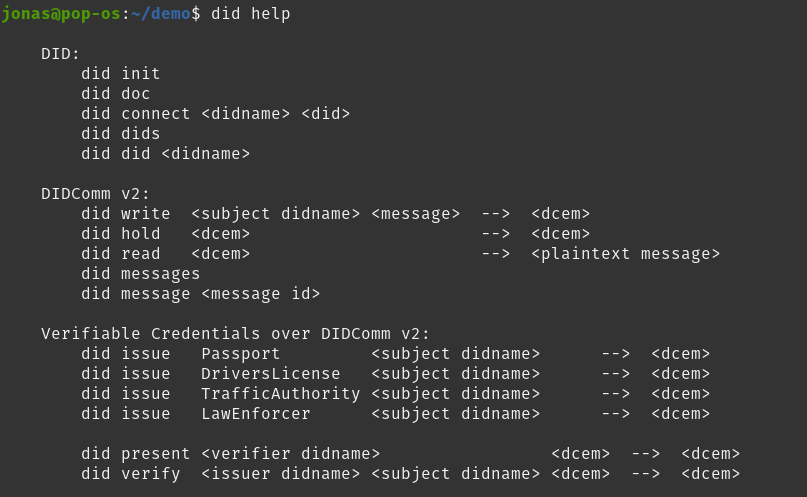
\includegraphics[width=.7\textwidth]{figures/cmd-help.png}
      \caption[]{Example running did help}
    \end{figure}
    
    
    
\subsection{did init}
\begin{itemize}
\item Creates an agent in the current directory.
\item The command creates a new `.did/`-directory, inside your working directory.
\item Your agents DID will be returned to `stdout` when running this command.
\item The command is idempotent.
\item \texttt{did init} bahaves almost identical to \texttt{git init}. This is intentional.
\end{itemize}
    \begin{figure}[htbp]
      \centering
      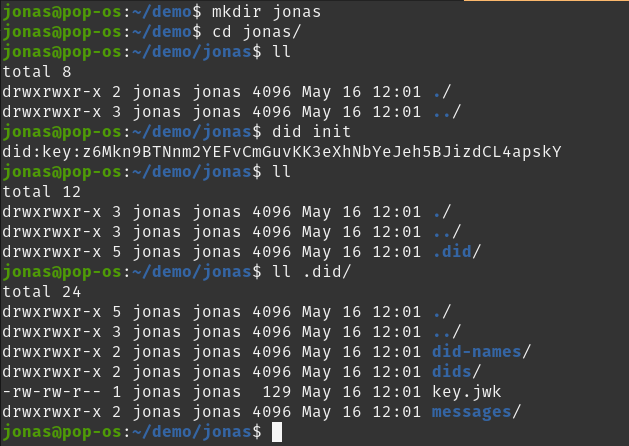
\includegraphics[width=.7\textwidth]{figures/cmd-init.png}
      \caption[]{Example running did init}
    \end{figure}
    


\subsection{did doc}
\begin{itemize}
\item Prints the did-document, controlled by the did agent.
\item Since the did-agent uses did-key as it's underlying did-method, the did-document is generated from the public-private keypair.
\item Another way to describe this is that did-key is self-resolving - the did-document is resolved directly from the did.
\item This is a limitation of the did-key method, and how it is specified.
\item Once created, the did-document pinned to a did-key did, is not possible to edit.
\end{itemize}
    \begin{figure}[htbp]
      \centering
      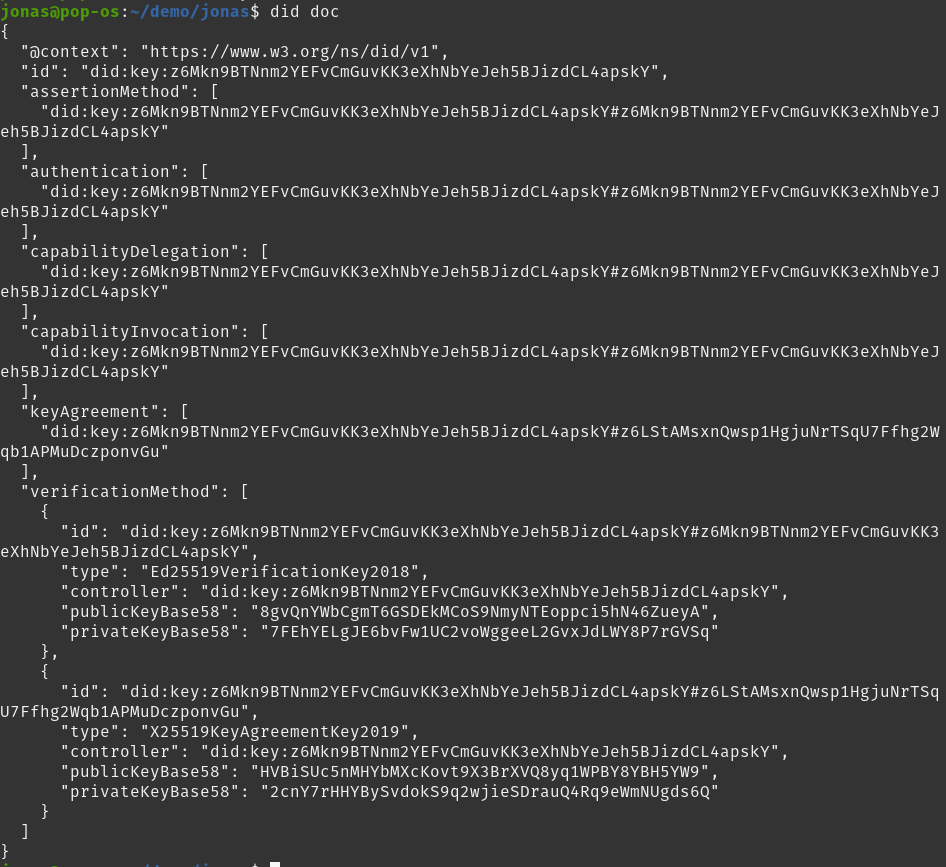
\includegraphics[width=.7\textwidth]{figures/cmd-doc.png}
      \caption[]{Example running did doc}
    \end{figure}



\subsection{did dids}
\begin{itemize}
\item List all dids stored in the agent.
\item Dids are added to the agent when running the `did connect` command.
\end{itemize}
    \begin{figure}[htbp]
      \centering
      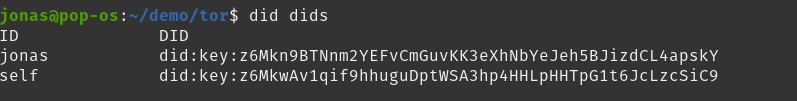
\includegraphics[width=.7\textwidth]{figures/cmd-dids.png}
      \caption[]{Example running did dids}
    \end{figure}



\subsection{did did <didname>}
\begin{itemize}
\item Show the did of a single `<didname>`.
\end{itemize}
    \begin{figure}[htbp]
      \centering
      
\includegraphics[width=.7\textwidth]{figures/cmd-did.png}
      \caption[]{Example running did did}
    \end{figure}



\subsection{did connect <didname> <did>}
\begin{itemize}
\item `did connect` connects a `<didname>` to `<did>`
\item `did connect` gives a `<did>` a `<didname>`.
\item The `<didname>` is used in other commands, as an easy way to refer to another agent's `<did>`.
\end{itemize}
    \begin{figure}[htbp]
      \centering
      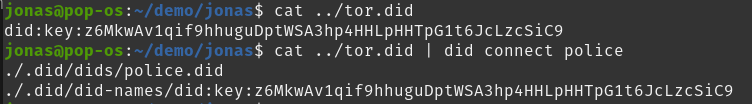
\includegraphics[width=.7\textwidth]{figures/cmd-connect.png}
      \caption[]{Example running did connect}
    \end{figure}



\subsection{did write <didname> <message>}
\begin{itemize}
\item Wraps a user defined message inside a `<dcem>`-envelope.
\item Sets the `to`-header of the `<dcem>` to the underlying `<did>` refered to by the `<didname>`.
\item Gives the message a new globally unique `id`.
\end{itemize}
    \begin{figure}[htbp]
      \centering
      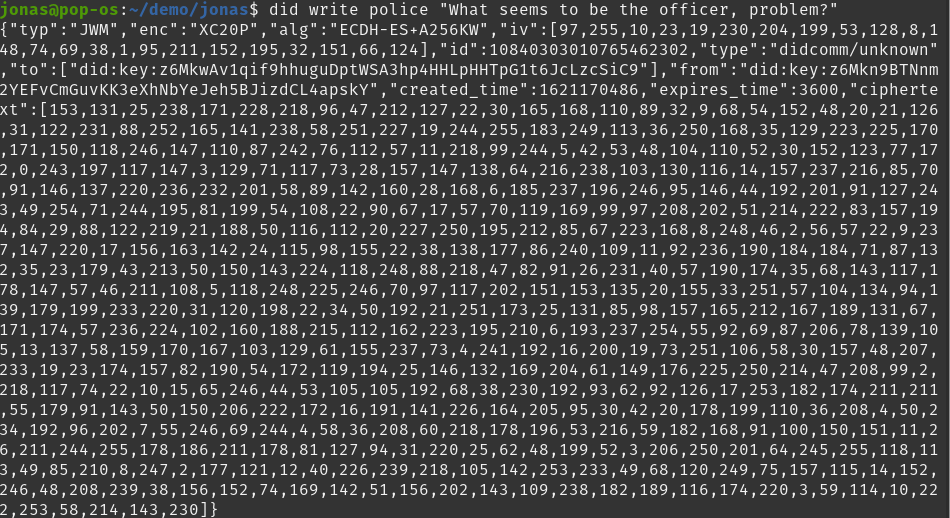
\includegraphics[width=.6\textwidth]{figures/cmd-write.png}
      \caption[]{Example running did write}
    \end{figure}
\newpage

\subsection{did read <dcem>}
\begin{itemize}
\item Unwraps an `<dcem>` message from `stdin` or from `<dcem>`-arg.
\item Prints the plaintext body of the message.
\end{itemize}
    \begin{figure}[htbp]
      \centering
      
\includegraphics[width=.65\textwidth]{figures/cmd-read-message.png}
      \caption[]{Example running did read <message>}
    \end{figure}
    \begin{figure}[htbp]
      \centering
      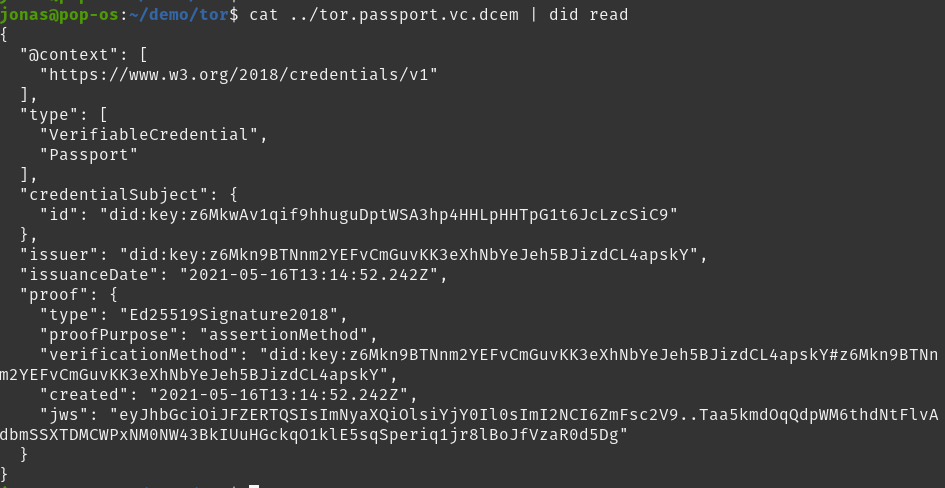
\includegraphics[width=.65\textwidth]{figures/cmd-read-vc.png}
      \caption[]{Example running did read <verifiable credential>}
    \end{figure}
    \begin{figure}[htbp]
      \centering
      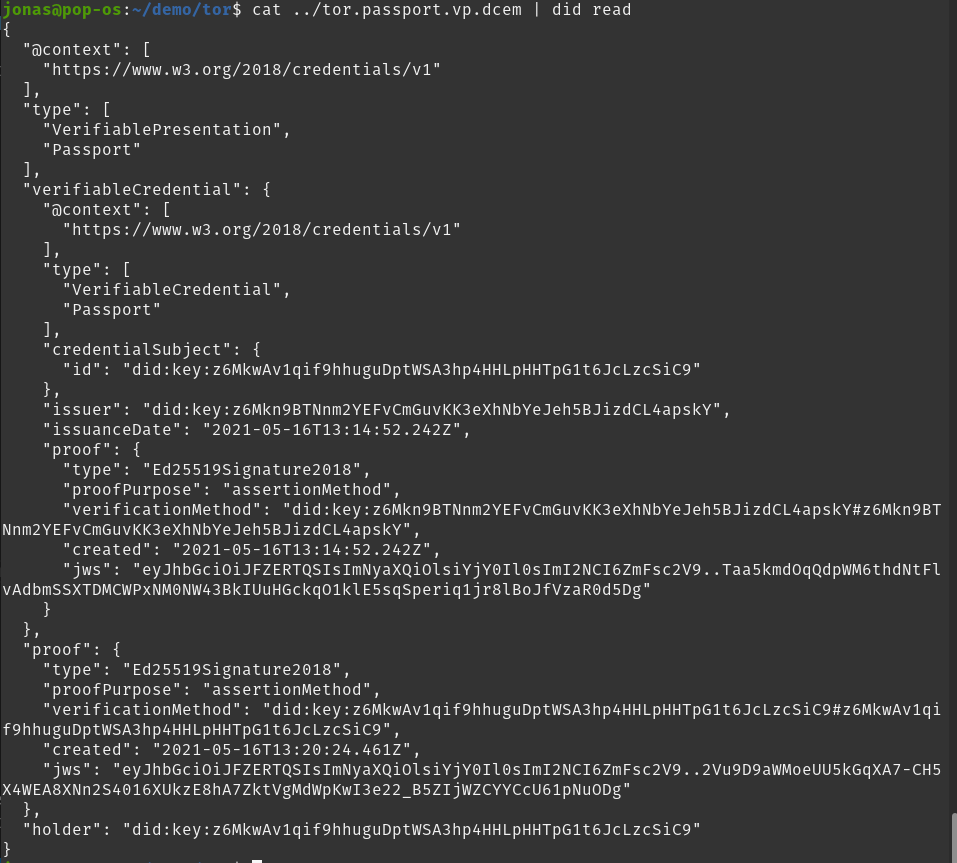
\includegraphics[width=.66\textwidth]{figures/cmd-read-vp.png}
      \caption[]{Example running did read <verifiable presentation>}
    \end{figure}

\newpage



\subsection{did issue <CredentialType> <didname>}
\begin{itemize}
\item Issues a verifiable credential addressed to the `did` of `<didname>`:
\item Issues one of 4 `<CredentialType>`s:
    \begin{itemize}
    \item Passport
    \item DriversLicense
    \item TrafficAuthority
    \item LawEnforcer
    \end{itemize}
\end{itemize}
    \begin{figure}[htbp]
      \centering
      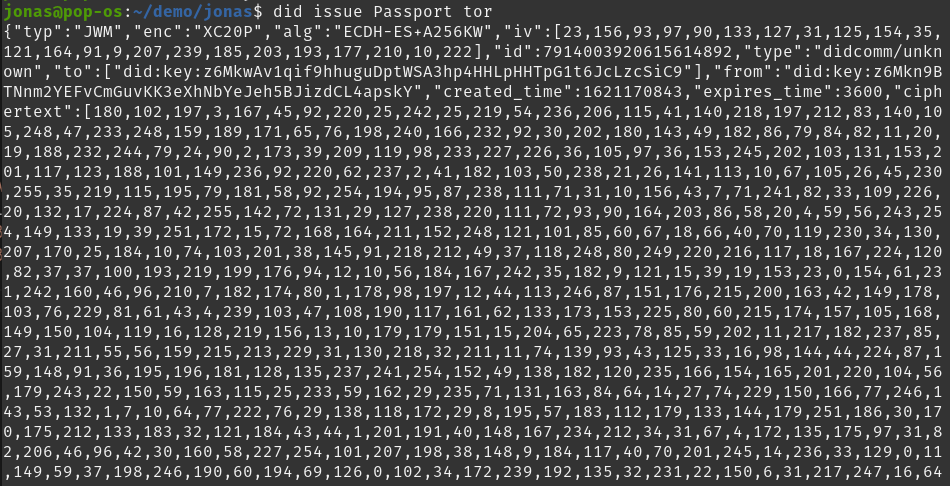
\includegraphics[width=.7\textwidth]{figures/cmd-issue.png}
      \caption[]{Example running did issue}
    \end{figure}



\subsection{did hold <dcem>}
\begin{itemize}
    \item Holds <dcem> and prints it to stdout
\end{itemize}
    \begin{figure}[htbp]
      \centering
      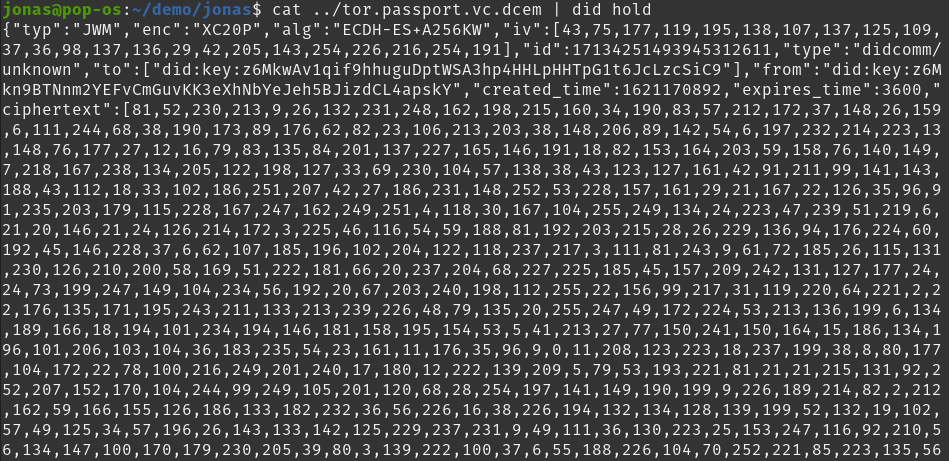
\includegraphics[width=.7\textwidth]{figures/cmd-hold.png}
      \caption[]{Example running did hold}
    \end{figure}

\newpage

\subsection{did present <didname> <dcem>}
\begin{itemize}
    \item Prints a Verifiable Presentation to stdout, with <dcem> as it's content 
\end{itemize}
    \begin{figure}[htbp]
      \centering
      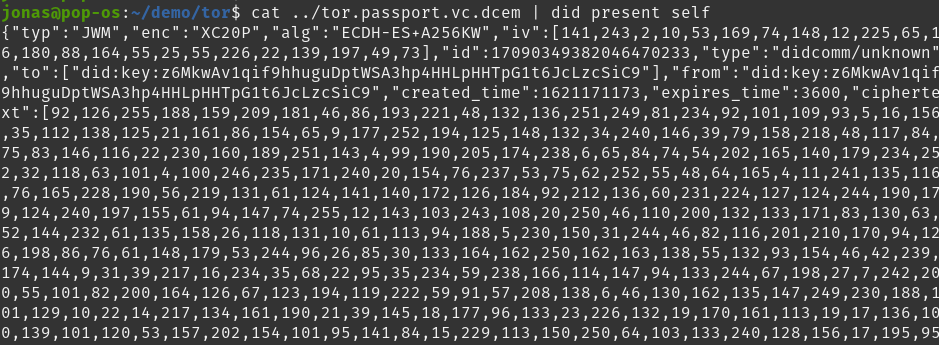
\includegraphics[width=.7\textwidth]{figures/cmd-present.png}
      \caption[]{Example running did present}
    \end{figure}


\subsection{did verify <issuer didname> <subject didname> <dcem>}
\begin{itemize}
\item Prints `<dcem>` to `stdout`, if, and only if, verification succeeds.
\end{itemize}
    \begin{figure}[htbp]
      \centering
      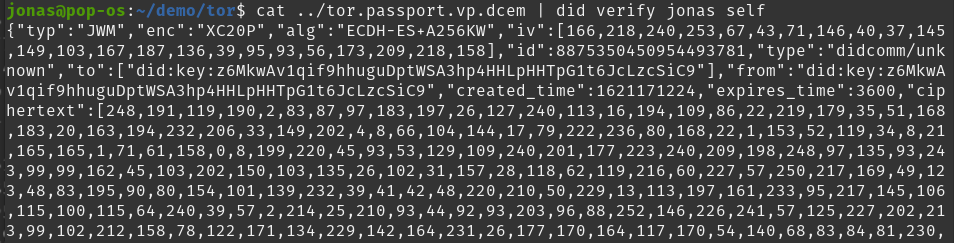
\includegraphics[width=.7\textwidth]{figures/cmd-verify.png}
      \caption[]{Example running did verify}
    \end{figure}
    \begin{figure}[htbp]
      \centering
      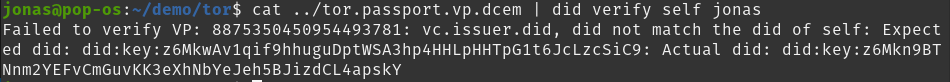
\includegraphics[width=.7\textwidth]{figures/cmd-verify-issuerfails.png}
      \caption[]{Example running did verify when issuer.did fails}
    \end{figure}


\newpage

\subsection{did messages}
\begin{itemize}
\item List all didcomm messages stored in the wallet.
\item Messages are added to the wallet when using the `did hold` command.
\end{itemize}
    \begin{figure}[htbp]
      \centering
      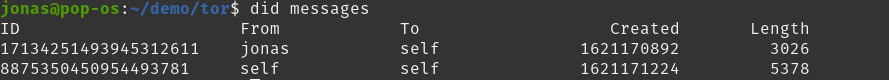
\includegraphics[width=.7\textwidth]{figures/cmd-messages.png}
      \caption[]{Example running did messages}
    \end{figure}

\subsection{did message <message id>}
\begin{itemize}
\item Show the contents of a single didcomm message based on the given `<message id>`.
\end{itemize}
    \begin{figure}[htbp]
      \centering
      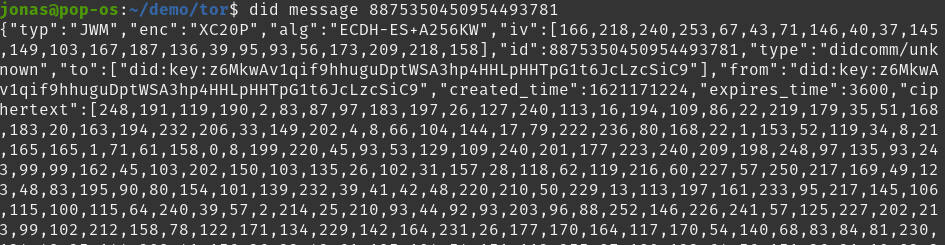
\includegraphics[width=.7\textwidth]{figures/cmd-message.png}
      \caption[]{Example running did message}
    \end{figure}

\section{Intentional limitations of the CLI}

\begin{itemize}
\item None of the commands have any optional-arguments - e.g `--option=<arg>`. This is to keep program logic as simple as possible. If the CLI was intended for a broader audicene with multiple use-cases, options may be added. This CLI is a special purpose CLI, intended to solve a specific use-case, namely the specific proof-of-concept from the problem statement. This is why optional-arguments was not prioritized.
\item Options are much harder to parse correctly than fixed size positional arguments.
\item None of the commands required variable length arguments, which made the implementation easier.
\item None of the commands have filepath arguments. The user is expected to use `cat <filepath>` to read the contents of a file, which is then fed into a positional argument of one of the commands. Example: `did read \$(cat ../message.dcem)` vs `did read ../message.dcem`. This was done to simplify implementation.
\end{itemize}
\chapter{Implementation}

\section{Code organization}

The source code is following the "guidelines for binary projects", given by the Rust-book, quoted in full below:


\paragraph{}
> Separation of Concerns for Binary Projects

\paragraph{}
> The organizational problem of allocating responsibility for multiple tasks to the main function is common to many binary projects. As a result, the Rust community has developed a process to use as a guideline for splitting the separate concerns of a binary program when main starts getting large. The process has the following steps:


\paragraph{}
>* Split your program into a main.rs and a lib.rs and move your program’s logic to lib.rs.
>* As long as your command line parsing logic is small, it can remain in main.rs.
>* When the command line parsing logic starts getting complicated, extract it from main.rs and move it to lib.rs.


\paragraph{}
>The responsibilities that remain in the main function after this process should be limited to the following:


\paragraph{}
>* Calling the command line parsing logic with the argument values
>* Setting up any other configuration
>* Calling a run function in lib.rs
>* Handling the error if run returns an error


\paragraph{}
>This pattern is about separating concerns: main.rs handles running the program, and lib.rs handles all the logic of the task at hand. Because you can’t test the main function directly, this structure lets you test all of your program’s logic by moving it into functions in lib.rs. The only code that remains in main.rs will be small enough to verify its correctness by reading it. Let’s rework our program by following this process.

\paragraph{}
Ref: https://doc.rust-lang.org/book/ch12-03-improving-error-handling-and-modularity.html\#separation-of-concerns-for-binary-projects


\subsection{File structure}


    \begin{figure}[htbp]
      \centering
      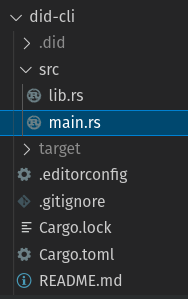
\includegraphics[width=.3\textwidth]{figures/code-organization.png}
      \caption[]{screenshot of the file-structure}
    \end{figure}

\subsection{Cargo package}

\begin{itemize}
    \item The source code is developed in the Rust programming language, as a Rust-package.
    \item There are two kinds of Rust-packages - binary packages (standalone executeables) and library packages (meant to be reused in other packages).
    \item Our Rust-package is named `did`, and is a binary package.
     All Rust-packages contains a `Cargo.toml` file, for stating metainfo about the source code.
    \item Here is a listing of the beginning of our [Cargo.toml](https://github.com/DIN-Foundation/bcs-ntnu-2021/blob/main/did-cli/Cargo.toml)
\end{itemize}
    
    \begin{lstlisting}[language=toml,caption={Cargo.toml}]
    
    [package]
    name = "did"
    version = "0.1.0"
    authors = ["Jonas Johan Solsvik <jonasjso@protonmail.com>"]
    edition = "2018"

    [dependencies]
    ...many things here
    \end{lstlisting}


\section{Build instructions}

\begin{itemize}
\item 1. Make sure you have installed the latest rust toolchain on your machine.

\begin{lstlisting}[language=bash,caption={From https://rustup.rs/}]
curl --proto '=https' --tlsv1.2 -sSf https://sh.rustup.rs | sh
\end{lstlisting}

\item 2. Clone from github source code

\begin{lstlisting}[language=bash,caption={}]
git clone git@github.com:DIN-Foundation/bcs-ntnu-2021.git
git submodule update --init --recursive
\end{lstlisting}


\item 3. Build the `did`-CLI using `cargo`

\begin{lstlisting}[language=bash,caption={}]
cd bcs-ntnu-2021/did-cli/
cargo build
\end{lstlisting}

\item 4. Copy the built executeable into some directory in your `\$PATH`.

\begin{lstlisting}[language=bash,caption={}]
cp target/debug/did \$HOME/bin/
\end{lstlisting}


\item 5. Run `did` by typing `did <command>` in your terminal.

\begin{lstlisting}[language=bash,caption={}]
did help
\end{lstlisting}
\end{itemize}



\section{Usage of existing Rust libraries}

\begin{description}
    \item[didcomm-rs:] Implements DIDComm v2 spec
    \item[spruceid/ssi:] Implements Verifiable Credentials spec
    \item[did-key.rs:] Implements DID-key method spec
    \item[ed25519-dalek:] Implements ed25519 public-private keypair management
\end{description}

\chapter{Quality Assurance}

\section{Manual testing}

When developing, most testing happens by manually running commands in the terminal, making sure they work correctly.
 
\section{Scenario Demonstration}

Demonstrating that DID CLI is able to solve the scenario put forth by the stakeholders, gives the team valuable feedback. The stakeholders will verify if the problem has been solved, and raise potential issues. This demonstration is an iterative process, and the stakeholders will receive the demonstration multiple times during development, to get as many iteration cycles as possible.
\chapter{Discussion}

\section{Summary}

?

\section{Talking to people about SSI}

A challenge that has surfaced during development, is how do you explain \acrshort{ssi} to people. A lot of different people have shown interest in this project during development. Here is a list of the different people, that need different explanations, based on their existing knowledge:

\begin{itemize}
    \item Parents
    \item Siblings
    \item Tech-savy-friends
    \item Non-tech-savy friends
    \item IT Colleagues
    \item University staff
\end{itemize}

\paragraph{}
Wired Magazine has a series of videos on youtube.com explaining a big concept in 5 levels of difficulty. One of their videos explains gravity in 5 levels\footnote{https://www.youtube.com/watch?v=QcUey-DVYjk}. This got me thinking: What Would a "5 levels of SSI"-video look like?

\paragraph{}
A list of concepts to get people "hooked":
\begin{itemize}
    \item Attester
    \item Vitnemål
    \item Kursbevis
    \item Kontrakter
    \item ID
    \item Skjøter
    \item Titler
    \item Fødselsattest
    \item Pass
    \item BankID
    \item Førerkort
    \item Bankkontoer
    \item Lånebevis
    \item Penger (cryptocurrency)
    \item Helsejournal - 200 different countries, 200 different helth care apps?
    \item Resepter
    \item ...and more
\end{itemize}


\section{Future Work}

?
\hypertarget{conclusion}{%
\chapter{Conclusion}\label{conclusion}}

\section{Summary}

In chapter 1 - Introduction - we laid out the current state of SSI and how SSI fits into the broader Web 3.0 ecosystem. We introduced the project and the team that would be working on it. Scopes and boundaries for the project where agreed upon.


\paragraph{}

In chapter 2 - Background - we explained the four layers of the SSI stack and that there are two broad categories of SSI applications - wallets and agents.


\paragraph{}
In chapter 3 - Development Process - we gave the reader insight into how the development of DID CLI was organized. We also revealed which tools where used - Kanban, Github, Discord, MS teams, Slack and Toggl.

  
\paragraph{}
In chapter 4 - Functional Requirements - The functional requirements of DID CLI was developed using a technique called Behaviour Driven Development (BDD). We systematically worked us through the four layers of the SSI stack, layer by layer.
  
  
\paragraph{}
In chapter 5 - User Interface - We get to experience how the user interface of DID CLI works and how it ties into the broader Unix ecosystem. The reader is presented with a list of all the available commands in DID CLI together with descriptions and screenshots of each command.


\paragraph{}
In chapter 6 - Architecture - An overview of DID-CLI the architecture is given. We also get more familiar with each component of the architecture. Also an analysis is given of the 4 external libraries which DID CLI depends on. We also learn how to install, build and RUN DID CLI. 


\paragraph{}
In chapter 7 - Results - We take a step back and look at what we were able to achieve by developing DID CLI. We learn that DID CLI was able to use existing Rust-libraries for most of it's core functionality. We learn that the novel approach of running DIDComm v2 over stdin/sdtout was a success and that by passing information via a Unix filesystem, 4 actors where able to create a network of SSI agents to simulate a real world scenario.


\paragraph{}
In chapter 8 - Discussion - We take a critical look on how this paper was developed. What went wrong? What is missing? What could have been done better and what we hope to achieve in the future projects.


\paragraph{}
Finally in chapter 9 - Conclusion - We do a summary and take a look on what the future holds for this very exciting field of computer engineering.

\section{Future work}

Since a core question of the problem description - "What is the state of interoperability in the SSI ecosystem?" - was not answered by this project, it is natural to suggest that this is something that could be picked up again in a later project.

"How does one go about testing the state of interoperability in SSI?" - you might ask. I think that the SSI ecosystem has a lot of potential learn from the rigorous engineering behind ensuring interoperability in the graphics industry. In computer graphics we have this thing called the Vulkan API\footnote{\url{https://www.khronos.org/registry/vulkan/specs/1.2-extensions/html/vkspec.html}}. The Vulkan API is not very different from things like DIDComm v2 in the SSI space, where Vulkan is a communication protocol between applications/games and the graphics hardware. To ensure interoperability between different hardware drivers - AMD, Nvidia or Intel - the Khronos group has put a lot of effort into \textit{The Vulkan Conformance Test suite(CTS)}\footnote{\url{https://github.com/KhronosGroup/VK-GL-CTS}}. This test suite ensures that you are able to swap your Nvidia card with an AMD card and be almost 100 percent confident that your Vulkan-application/game still work.

In my opinion the SSI space needs it's own conformance test suite(CTS) for DIDComm v2, to ensure DIDComm v2 "drivers" actually stick to the rules. Only then can we grow the engineering confidence that serious applications could be built on top of it. We already have things like this in the SSI space. I am specifically thinking of \textit{The Aries interop test suite}\footnote{\url{https://github.com/hyperledger/aries-protocol-test-suite}}. Now what is Aries? Aries is the reason why DIDComm v2 has the v2 suffix. Because Aries is considered to be DIDComm v1\footnote{\url{https://github.com/hyperledger/aries-rfcs/blob/main/concepts/0005-didcomm/README.md}}.


\chapter*{\bibname}
\printbibliography[heading=none]

%\appendix
%\input{appendices/a-appendix.tex}

\end{document}
